\documentclass{article}
\usepackage[final]{neurips_2025}  % NEURIPS style (neurips_2025.sty is in paper_draft/)
% [final] alone leaves the track name undefined in neurips_2025.sty; default to the main track
\makeatletter\providecommand{\@trackname}{\@neuripsordinal\ Conference on Neural Information Processing Systems (NeurIPS \@neuripsyear).}\makeatother
\usepackage[hidelinks]{hyperref}  % REQUIRED: clickable links
\usepackage{booktabs}  % REQUIRED: professional tables
\usepackage{graphicx}
\usepackage{amsmath,amssymb}

\usepackage[utf8]{inputenc}
\usepackage[T1]{fontenc}
\usepackage{xspace}
\usepackage{enumitem}
\usepackage{multirow}
\usepackage{subcaption}
\usepackage{algorithm}
\usepackage[noend]{algpseudocode}

% Import command files
%%%%% MATH NOTATION MACROS %%%%%
% Standard math notation for academic papers
% Import with: %%%%% MATH NOTATION MACROS %%%%%
% Standard math notation for academic papers
% Import with: %%%%% MATH NOTATION MACROS %%%%%
% Standard math notation for academic papers
% Import with: \input{commands/math}

\usepackage{amsmath,amsfonts,bm}

%%%%%%%%%%%%%%%%%%%%%%%%%%%%%%%%%%%%%%%%%%%%%%%%%%%%%%%%%%%%%%%%%
% FIGURE AND SECTION REFERENCES
%%%%%%%%%%%%%%%%%%%%%%%%%%%%%%%%%%%%%%%%%%%%%%%%%%%%%%%%%%%%%%%%%

% Mark sections of captions for referring to divisions of figures
\newcommand{\figleft}{{\em (Left)}}
\newcommand{\figcenter}{{\em (Center)}}
\newcommand{\figright}{{\em (Right)}}
\newcommand{\figtop}{{\em (Top)}}
\newcommand{\figbottom}{{\em (Bottom)}}
\newcommand{\captiona}{{\em (a)}}
\newcommand{\captionb}{{\em (b)}}
\newcommand{\captionc}{{\em (c)}}
\newcommand{\captiond}{{\em (d)}}

% Figure references
\def\figref#1{figure~\ref{#1}}
\def\Figref#1{Figure~\ref{#1}}
\def\twofigref#1#2{figures \ref{#1} and \ref{#2}}
\def\quadfigref#1#2#3#4{figures \ref{#1}, \ref{#2}, \ref{#3} and \ref{#4}}

% Section references
\def\secref#1{section~\ref{#1}}
\def\Secref#1{Section~\ref{#1}}
\def\twosecrefs#1#2{sections \ref{#1} and \ref{#2}}
\def\secrefs#1#2#3{sections \ref{#1}, \ref{#2} and \ref{#3}}

% Equation references
\def\eqref#1{equation~\ref{#1}}
\def\Eqref#1{Equation~\ref{#1}}
\def\plaineqref#1{\ref{#1}}

% Algorithm references
\def\algref#1{algorithm~\ref{#1}}
\def\Algref#1{Algorithm~\ref{#1}}
\def\twoalgref#1#2{algorithms \ref{#1} and \ref{#2}}
\def\Twoalgref#1#2{Algorithms \ref{#1} and \ref{#2}}

% Table references
\def\tabref#1{table~\ref{#1}}
\def\Tabref#1{Table~\ref{#1}}

% Chapter references
\def\chapref#1{chapter~\ref{#1}}
\def\Chapref#1{Chapter~\ref{#1}}

%%%%%%%%%%%%%%%%%%%%%%%%%%%%%%%%%%%%%%%%%%%%%%%%%%%%%%%%%%%%%%%%%
% BASIC MATH DEFINITIONS
%%%%%%%%%%%%%%%%%%%%%%%%%%%%%%%%%%%%%%%%%%%%%%%%%%%%%%%%%%%%%%%%%

\def\ceil#1{\lceil #1 \rceil}
\def\floor#1{\lfloor #1 \rfloor}
\def\1{\bm{1}}
\def\eps{{\epsilon}}

% Common operators
\DeclareMathOperator*{\argmax}{arg\,max}
\DeclareMathOperator*{\argmin}{arg\,min}
\DeclareMathOperator{\sign}{sign}
\DeclareMathOperator{\Tr}{Tr}
\let\ab\allowbreak

%%%%%%%%%%%%%%%%%%%%%%%%%%%%%%%%%%%%%%%%%%%%%%%%%%%%%%%%%%%%%%%%%
% VECTORS (lowercase bold)
%%%%%%%%%%%%%%%%%%%%%%%%%%%%%%%%%%%%%%%%%%%%%%%%%%%%%%%%%%%%%%%%%

\def\vzero{{\bm{0}}}
\def\vone{{\bm{1}}}
\def\vmu{{\bm{\mu}}}
\def\vtheta{{\bm{\theta}}}
\def\va{{\bm{a}}}
\def\vb{{\bm{b}}}
\def\vc{{\bm{c}}}
\def\vd{{\bm{d}}}
\def\ve{{\bm{e}}}
\def\vf{{\bm{f}}}
\def\vg{{\bm{g}}}
\def\vh{{\bm{h}}}
\def\vi{{\bm{i}}}
\def\vj{{\bm{j}}}
\def\vk{{\bm{k}}}
\def\vl{{\bm{l}}}
\def\vm{{\bm{m}}}
\def\vn{{\bm{n}}}
\def\vo{{\bm{o}}}
\def\vp{{\bm{p}}}
\def\vq{{\bm{q}}}
\def\vr{{\bm{r}}}
\def\vs{{\bm{s}}}
\def\vt{{\bm{t}}}
\def\vu{{\bm{u}}}
\def\vv{{\bm{v}}}
\def\vw{{\bm{w}}}
\def\vx{{\bm{x}}}
\def\vy{{\bm{y}}}
\def\vz{{\bm{z}}}

%%%%%%%%%%%%%%%%%%%%%%%%%%%%%%%%%%%%%%%%%%%%%%%%%%%%%%%%%%%%%%%%%
% MATRICES (uppercase bold)
%%%%%%%%%%%%%%%%%%%%%%%%%%%%%%%%%%%%%%%%%%%%%%%%%%%%%%%%%%%%%%%%%

\def\mA{{\bm{A}}}
\def\mB{{\bm{B}}}
\def\mC{{\bm{C}}}
\def\mD{{\bm{D}}}
\def\mE{{\bm{E}}}
\def\mF{{\bm{F}}}
\def\mG{{\bm{G}}}
\def\mH{{\bm{H}}}
\def\mI{{\bm{I}}}
\def\mJ{{\bm{J}}}
\def\mK{{\bm{K}}}
\def\mL{{\bm{L}}}
\def\mM{{\bm{M}}}
\def\mN{{\bm{N}}}
\def\mO{{\bm{O}}}
\def\mP{{\bm{P}}}
\def\mQ{{\bm{Q}}}
\def\mR{{\bm{R}}}
\def\mS{{\bm{S}}}
\def\mT{{\bm{T}}}
\def\mU{{\bm{U}}}
\def\mV{{\bm{V}}}
\def\mW{{\bm{W}}}
\def\mX{{\bm{X}}}
\def\mY{{\bm{Y}}}
\def\mZ{{\bm{Z}}}
\def\mBeta{{\bm{\beta}}}
\def\mPhi{{\bm{\Phi}}}
\def\mLambda{{\bm{\Lambda}}}
\def\mSigma{{\bm{\Sigma}}}

%%%%%%%%%%%%%%%%%%%%%%%%%%%%%%%%%%%%%%%%%%%%%%%%%%%%%%%%%%%%%%%%%
% CALLIGRAPHIC (mathcal)
%%%%%%%%%%%%%%%%%%%%%%%%%%%%%%%%%%%%%%%%%%%%%%%%%%%%%%%%%%%%%%%%%

\def\gA{{\mathcal{A}}}
\def\gB{{\mathcal{B}}}
\def\gC{{\mathcal{C}}}
\def\gD{{\mathcal{D}}}
\def\gE{{\mathcal{E}}}
\def\gF{{\mathcal{F}}}
\def\gG{{\mathcal{G}}}
\def\gH{{\mathcal{H}}}
\def\gI{{\mathcal{I}}}
\def\gJ{{\mathcal{J}}}
\def\gK{{\mathcal{K}}}
\def\gL{{\mathcal{L}}}
\def\gM{{\mathcal{M}}}
\def\gN{{\mathcal{N}}}
\def\gO{{\mathcal{O}}}
\def\gP{{\mathcal{P}}}
\def\gQ{{\mathcal{Q}}}
\def\gR{{\mathcal{R}}}
\def\gS{{\mathcal{S}}}
\def\gT{{\mathcal{T}}}
\def\gU{{\mathcal{U}}}
\def\gV{{\mathcal{V}}}
\def\gW{{\mathcal{W}}}
\def\gX{{\mathcal{X}}}
\def\gY{{\mathcal{Y}}}
\def\gZ{{\mathcal{Z}}}

%%%%%%%%%%%%%%%%%%%%%%%%%%%%%%%%%%%%%%%%%%%%%%%%%%%%%%%%%%%%%%%%%
% SETS (blackboard bold)
%%%%%%%%%%%%%%%%%%%%%%%%%%%%%%%%%%%%%%%%%%%%%%%%%%%%%%%%%%%%%%%%%

\def\sA{{\mathbb{A}}}
\def\sB{{\mathbb{B}}}
\def\sC{{\mathbb{C}}}
\def\sD{{\mathbb{D}}}
\def\sF{{\mathbb{F}}}
\def\sG{{\mathbb{G}}}
\def\sH{{\mathbb{H}}}
\def\sI{{\mathbb{I}}}
\def\sJ{{\mathbb{J}}}
\def\sK{{\mathbb{K}}}
\def\sL{{\mathbb{L}}}
\def\sM{{\mathbb{M}}}
\def\sN{{\mathbb{N}}}
\def\sO{{\mathbb{O}}}
\def\sP{{\mathbb{P}}}
\def\sQ{{\mathbb{Q}}}
\def\sR{{\mathbb{R}}}
\def\sS{{\mathbb{S}}}
\def\sT{{\mathbb{T}}}
\def\sU{{\mathbb{U}}}
\def\sV{{\mathbb{V}}}
\def\sW{{\mathbb{W}}}
\def\sX{{\mathbb{X}}}
\def\sY{{\mathbb{Y}}}
\def\sZ{{\mathbb{Z}}}

%%%%%%%%%%%%%%%%%%%%%%%%%%%%%%%%%%%%%%%%%%%%%%%%%%%%%%%%%%%%%%%%%
% COMMON MATH SHORTCUTS
%%%%%%%%%%%%%%%%%%%%%%%%%%%%%%%%%%%%%%%%%%%%%%%%%%%%%%%%%%%%%%%%%

% Expectation and variance
\newcommand{\E}{\mathbb{E}}
\newcommand{\Var}{\mathrm{Var}}
\newcommand{\Cov}{\mathrm{Cov}}
\newcommand{\R}{\mathbb{R}}

% Datasets
\newcommand{\train}{\mathcal{D}}
\newcommand{\valid}{\mathcal{D_{\mathrm{valid}}}}
\newcommand{\test}{\mathcal{D_{\mathrm{test}}}}

% Distributions
\newcommand{\laplace}{\mathrm{Laplace}}
\newcommand{\Uniform}{\mathrm{Unif}}
\newcommand{\Normal}{\mathrm{Normal}}
\newcommand{\Categorical}{\mathrm{Categorical}}

% Common functions
\newcommand{\softmax}{\mathrm{softmax}}
\newcommand{\sigmoid}{\sigma}
\newcommand{\KL}{D_{\mathrm{KL}}}

% Norms
\newcommand{\normlzero}{L^0}
\newcommand{\normlone}{L^1}
\newcommand{\normltwo}{L^2}
\newcommand{\normlp}{L^p}
\newcommand{\normmax}{L^\infty}

%%%%%%%%%%%%%%%%%%%%%%%%%%%%%%%%%%%%%%%%%%%%%%%%%%%%%%%%%%%%%%%%%
% DEFINITIONS AND HIGHLIGHTING
%%%%%%%%%%%%%%%%%%%%%%%%%%%%%%%%%%%%%%%%%%%%%%%%%%%%%%%%%%%%%%%%%

% Highlight a newly defined term
\newcommand{\newterm}[1]{{\bf #1}}
\newcommand{\defn}[1]{\textbf{#1}}
\newcommand{\defeq}{\mathrel{\stackrel{\textnormal{\tiny def}}{=}}}


\usepackage{amsmath,amsfonts,bm}

%%%%%%%%%%%%%%%%%%%%%%%%%%%%%%%%%%%%%%%%%%%%%%%%%%%%%%%%%%%%%%%%%
% FIGURE AND SECTION REFERENCES
%%%%%%%%%%%%%%%%%%%%%%%%%%%%%%%%%%%%%%%%%%%%%%%%%%%%%%%%%%%%%%%%%

% Mark sections of captions for referring to divisions of figures
\newcommand{\figleft}{{\em (Left)}}
\newcommand{\figcenter}{{\em (Center)}}
\newcommand{\figright}{{\em (Right)}}
\newcommand{\figtop}{{\em (Top)}}
\newcommand{\figbottom}{{\em (Bottom)}}
\newcommand{\captiona}{{\em (a)}}
\newcommand{\captionb}{{\em (b)}}
\newcommand{\captionc}{{\em (c)}}
\newcommand{\captiond}{{\em (d)}}

% Figure references
\def\figref#1{figure~\ref{#1}}
\def\Figref#1{Figure~\ref{#1}}
\def\twofigref#1#2{figures \ref{#1} and \ref{#2}}
\def\quadfigref#1#2#3#4{figures \ref{#1}, \ref{#2}, \ref{#3} and \ref{#4}}

% Section references
\def\secref#1{section~\ref{#1}}
\def\Secref#1{Section~\ref{#1}}
\def\twosecrefs#1#2{sections \ref{#1} and \ref{#2}}
\def\secrefs#1#2#3{sections \ref{#1}, \ref{#2} and \ref{#3}}

% Equation references
\def\eqref#1{equation~\ref{#1}}
\def\Eqref#1{Equation~\ref{#1}}
\def\plaineqref#1{\ref{#1}}

% Algorithm references
\def\algref#1{algorithm~\ref{#1}}
\def\Algref#1{Algorithm~\ref{#1}}
\def\twoalgref#1#2{algorithms \ref{#1} and \ref{#2}}
\def\Twoalgref#1#2{Algorithms \ref{#1} and \ref{#2}}

% Table references
\def\tabref#1{table~\ref{#1}}
\def\Tabref#1{Table~\ref{#1}}

% Chapter references
\def\chapref#1{chapter~\ref{#1}}
\def\Chapref#1{Chapter~\ref{#1}}

%%%%%%%%%%%%%%%%%%%%%%%%%%%%%%%%%%%%%%%%%%%%%%%%%%%%%%%%%%%%%%%%%
% BASIC MATH DEFINITIONS
%%%%%%%%%%%%%%%%%%%%%%%%%%%%%%%%%%%%%%%%%%%%%%%%%%%%%%%%%%%%%%%%%

\def\ceil#1{\lceil #1 \rceil}
\def\floor#1{\lfloor #1 \rfloor}
\def\1{\bm{1}}
\def\eps{{\epsilon}}

% Common operators
\DeclareMathOperator*{\argmax}{arg\,max}
\DeclareMathOperator*{\argmin}{arg\,min}
\DeclareMathOperator{\sign}{sign}
\DeclareMathOperator{\Tr}{Tr}
\let\ab\allowbreak

%%%%%%%%%%%%%%%%%%%%%%%%%%%%%%%%%%%%%%%%%%%%%%%%%%%%%%%%%%%%%%%%%
% VECTORS (lowercase bold)
%%%%%%%%%%%%%%%%%%%%%%%%%%%%%%%%%%%%%%%%%%%%%%%%%%%%%%%%%%%%%%%%%

\def\vzero{{\bm{0}}}
\def\vone{{\bm{1}}}
\def\vmu{{\bm{\mu}}}
\def\vtheta{{\bm{\theta}}}
\def\va{{\bm{a}}}
\def\vb{{\bm{b}}}
\def\vc{{\bm{c}}}
\def\vd{{\bm{d}}}
\def\ve{{\bm{e}}}
\def\vf{{\bm{f}}}
\def\vg{{\bm{g}}}
\def\vh{{\bm{h}}}
\def\vi{{\bm{i}}}
\def\vj{{\bm{j}}}
\def\vk{{\bm{k}}}
\def\vl{{\bm{l}}}
\def\vm{{\bm{m}}}
\def\vn{{\bm{n}}}
\def\vo{{\bm{o}}}
\def\vp{{\bm{p}}}
\def\vq{{\bm{q}}}
\def\vr{{\bm{r}}}
\def\vs{{\bm{s}}}
\def\vt{{\bm{t}}}
\def\vu{{\bm{u}}}
\def\vv{{\bm{v}}}
\def\vw{{\bm{w}}}
\def\vx{{\bm{x}}}
\def\vy{{\bm{y}}}
\def\vz{{\bm{z}}}

%%%%%%%%%%%%%%%%%%%%%%%%%%%%%%%%%%%%%%%%%%%%%%%%%%%%%%%%%%%%%%%%%
% MATRICES (uppercase bold)
%%%%%%%%%%%%%%%%%%%%%%%%%%%%%%%%%%%%%%%%%%%%%%%%%%%%%%%%%%%%%%%%%

\def\mA{{\bm{A}}}
\def\mB{{\bm{B}}}
\def\mC{{\bm{C}}}
\def\mD{{\bm{D}}}
\def\mE{{\bm{E}}}
\def\mF{{\bm{F}}}
\def\mG{{\bm{G}}}
\def\mH{{\bm{H}}}
\def\mI{{\bm{I}}}
\def\mJ{{\bm{J}}}
\def\mK{{\bm{K}}}
\def\mL{{\bm{L}}}
\def\mM{{\bm{M}}}
\def\mN{{\bm{N}}}
\def\mO{{\bm{O}}}
\def\mP{{\bm{P}}}
\def\mQ{{\bm{Q}}}
\def\mR{{\bm{R}}}
\def\mS{{\bm{S}}}
\def\mT{{\bm{T}}}
\def\mU{{\bm{U}}}
\def\mV{{\bm{V}}}
\def\mW{{\bm{W}}}
\def\mX{{\bm{X}}}
\def\mY{{\bm{Y}}}
\def\mZ{{\bm{Z}}}
\def\mBeta{{\bm{\beta}}}
\def\mPhi{{\bm{\Phi}}}
\def\mLambda{{\bm{\Lambda}}}
\def\mSigma{{\bm{\Sigma}}}

%%%%%%%%%%%%%%%%%%%%%%%%%%%%%%%%%%%%%%%%%%%%%%%%%%%%%%%%%%%%%%%%%
% CALLIGRAPHIC (mathcal)
%%%%%%%%%%%%%%%%%%%%%%%%%%%%%%%%%%%%%%%%%%%%%%%%%%%%%%%%%%%%%%%%%

\def\gA{{\mathcal{A}}}
\def\gB{{\mathcal{B}}}
\def\gC{{\mathcal{C}}}
\def\gD{{\mathcal{D}}}
\def\gE{{\mathcal{E}}}
\def\gF{{\mathcal{F}}}
\def\gG{{\mathcal{G}}}
\def\gH{{\mathcal{H}}}
\def\gI{{\mathcal{I}}}
\def\gJ{{\mathcal{J}}}
\def\gK{{\mathcal{K}}}
\def\gL{{\mathcal{L}}}
\def\gM{{\mathcal{M}}}
\def\gN{{\mathcal{N}}}
\def\gO{{\mathcal{O}}}
\def\gP{{\mathcal{P}}}
\def\gQ{{\mathcal{Q}}}
\def\gR{{\mathcal{R}}}
\def\gS{{\mathcal{S}}}
\def\gT{{\mathcal{T}}}
\def\gU{{\mathcal{U}}}
\def\gV{{\mathcal{V}}}
\def\gW{{\mathcal{W}}}
\def\gX{{\mathcal{X}}}
\def\gY{{\mathcal{Y}}}
\def\gZ{{\mathcal{Z}}}

%%%%%%%%%%%%%%%%%%%%%%%%%%%%%%%%%%%%%%%%%%%%%%%%%%%%%%%%%%%%%%%%%
% SETS (blackboard bold)
%%%%%%%%%%%%%%%%%%%%%%%%%%%%%%%%%%%%%%%%%%%%%%%%%%%%%%%%%%%%%%%%%

\def\sA{{\mathbb{A}}}
\def\sB{{\mathbb{B}}}
\def\sC{{\mathbb{C}}}
\def\sD{{\mathbb{D}}}
\def\sF{{\mathbb{F}}}
\def\sG{{\mathbb{G}}}
\def\sH{{\mathbb{H}}}
\def\sI{{\mathbb{I}}}
\def\sJ{{\mathbb{J}}}
\def\sK{{\mathbb{K}}}
\def\sL{{\mathbb{L}}}
\def\sM{{\mathbb{M}}}
\def\sN{{\mathbb{N}}}
\def\sO{{\mathbb{O}}}
\def\sP{{\mathbb{P}}}
\def\sQ{{\mathbb{Q}}}
\def\sR{{\mathbb{R}}}
\def\sS{{\mathbb{S}}}
\def\sT{{\mathbb{T}}}
\def\sU{{\mathbb{U}}}
\def\sV{{\mathbb{V}}}
\def\sW{{\mathbb{W}}}
\def\sX{{\mathbb{X}}}
\def\sY{{\mathbb{Y}}}
\def\sZ{{\mathbb{Z}}}

%%%%%%%%%%%%%%%%%%%%%%%%%%%%%%%%%%%%%%%%%%%%%%%%%%%%%%%%%%%%%%%%%
% COMMON MATH SHORTCUTS
%%%%%%%%%%%%%%%%%%%%%%%%%%%%%%%%%%%%%%%%%%%%%%%%%%%%%%%%%%%%%%%%%

% Expectation and variance
\newcommand{\E}{\mathbb{E}}
\newcommand{\Var}{\mathrm{Var}}
\newcommand{\Cov}{\mathrm{Cov}}
\newcommand{\R}{\mathbb{R}}

% Datasets
\newcommand{\train}{\mathcal{D}}
\newcommand{\valid}{\mathcal{D_{\mathrm{valid}}}}
\newcommand{\test}{\mathcal{D_{\mathrm{test}}}}

% Distributions
\newcommand{\laplace}{\mathrm{Laplace}}
\newcommand{\Uniform}{\mathrm{Unif}}
\newcommand{\Normal}{\mathrm{Normal}}
\newcommand{\Categorical}{\mathrm{Categorical}}

% Common functions
\newcommand{\softmax}{\mathrm{softmax}}
\newcommand{\sigmoid}{\sigma}
\newcommand{\KL}{D_{\mathrm{KL}}}

% Norms
\newcommand{\normlzero}{L^0}
\newcommand{\normlone}{L^1}
\newcommand{\normltwo}{L^2}
\newcommand{\normlp}{L^p}
\newcommand{\normmax}{L^\infty}

%%%%%%%%%%%%%%%%%%%%%%%%%%%%%%%%%%%%%%%%%%%%%%%%%%%%%%%%%%%%%%%%%
% DEFINITIONS AND HIGHLIGHTING
%%%%%%%%%%%%%%%%%%%%%%%%%%%%%%%%%%%%%%%%%%%%%%%%%%%%%%%%%%%%%%%%%

% Highlight a newly defined term
\newcommand{\newterm}[1]{{\bf #1}}
\newcommand{\defn}[1]{\textbf{#1}}
\newcommand{\defeq}{\mathrel{\stackrel{\textnormal{\tiny def}}{=}}}


\usepackage{amsmath,amsfonts,bm}

%%%%%%%%%%%%%%%%%%%%%%%%%%%%%%%%%%%%%%%%%%%%%%%%%%%%%%%%%%%%%%%%%
% FIGURE AND SECTION REFERENCES
%%%%%%%%%%%%%%%%%%%%%%%%%%%%%%%%%%%%%%%%%%%%%%%%%%%%%%%%%%%%%%%%%

% Mark sections of captions for referring to divisions of figures
\newcommand{\figleft}{{\em (Left)}}
\newcommand{\figcenter}{{\em (Center)}}
\newcommand{\figright}{{\em (Right)}}
\newcommand{\figtop}{{\em (Top)}}
\newcommand{\figbottom}{{\em (Bottom)}}
\newcommand{\captiona}{{\em (a)}}
\newcommand{\captionb}{{\em (b)}}
\newcommand{\captionc}{{\em (c)}}
\newcommand{\captiond}{{\em (d)}}

% Figure references
\def\figref#1{figure~\ref{#1}}
\def\Figref#1{Figure~\ref{#1}}
\def\twofigref#1#2{figures \ref{#1} and \ref{#2}}
\def\quadfigref#1#2#3#4{figures \ref{#1}, \ref{#2}, \ref{#3} and \ref{#4}}

% Section references
\def\secref#1{section~\ref{#1}}
\def\Secref#1{Section~\ref{#1}}
\def\twosecrefs#1#2{sections \ref{#1} and \ref{#2}}
\def\secrefs#1#2#3{sections \ref{#1}, \ref{#2} and \ref{#3}}

% Equation references
\def\eqref#1{equation~\ref{#1}}
\def\Eqref#1{Equation~\ref{#1}}
\def\plaineqref#1{\ref{#1}}

% Algorithm references
\def\algref#1{algorithm~\ref{#1}}
\def\Algref#1{Algorithm~\ref{#1}}
\def\twoalgref#1#2{algorithms \ref{#1} and \ref{#2}}
\def\Twoalgref#1#2{Algorithms \ref{#1} and \ref{#2}}

% Table references
\def\tabref#1{table~\ref{#1}}
\def\Tabref#1{Table~\ref{#1}}

% Chapter references
\def\chapref#1{chapter~\ref{#1}}
\def\Chapref#1{Chapter~\ref{#1}}

%%%%%%%%%%%%%%%%%%%%%%%%%%%%%%%%%%%%%%%%%%%%%%%%%%%%%%%%%%%%%%%%%
% BASIC MATH DEFINITIONS
%%%%%%%%%%%%%%%%%%%%%%%%%%%%%%%%%%%%%%%%%%%%%%%%%%%%%%%%%%%%%%%%%

\def\ceil#1{\lceil #1 \rceil}
\def\floor#1{\lfloor #1 \rfloor}
\def\1{\bm{1}}
\def\eps{{\epsilon}}

% Common operators
\DeclareMathOperator*{\argmax}{arg\,max}
\DeclareMathOperator*{\argmin}{arg\,min}
\DeclareMathOperator{\sign}{sign}
\DeclareMathOperator{\Tr}{Tr}
\let\ab\allowbreak

%%%%%%%%%%%%%%%%%%%%%%%%%%%%%%%%%%%%%%%%%%%%%%%%%%%%%%%%%%%%%%%%%
% VECTORS (lowercase bold)
%%%%%%%%%%%%%%%%%%%%%%%%%%%%%%%%%%%%%%%%%%%%%%%%%%%%%%%%%%%%%%%%%

\def\vzero{{\bm{0}}}
\def\vone{{\bm{1}}}
\def\vmu{{\bm{\mu}}}
\def\vtheta{{\bm{\theta}}}
\def\va{{\bm{a}}}
\def\vb{{\bm{b}}}
\def\vc{{\bm{c}}}
\def\vd{{\bm{d}}}
\def\ve{{\bm{e}}}
\def\vf{{\bm{f}}}
\def\vg{{\bm{g}}}
\def\vh{{\bm{h}}}
\def\vi{{\bm{i}}}
\def\vj{{\bm{j}}}
\def\vk{{\bm{k}}}
\def\vl{{\bm{l}}}
\def\vm{{\bm{m}}}
\def\vn{{\bm{n}}}
\def\vo{{\bm{o}}}
\def\vp{{\bm{p}}}
\def\vq{{\bm{q}}}
\def\vr{{\bm{r}}}
\def\vs{{\bm{s}}}
\def\vt{{\bm{t}}}
\def\vu{{\bm{u}}}
\def\vv{{\bm{v}}}
\def\vw{{\bm{w}}}
\def\vx{{\bm{x}}}
\def\vy{{\bm{y}}}
\def\vz{{\bm{z}}}

%%%%%%%%%%%%%%%%%%%%%%%%%%%%%%%%%%%%%%%%%%%%%%%%%%%%%%%%%%%%%%%%%
% MATRICES (uppercase bold)
%%%%%%%%%%%%%%%%%%%%%%%%%%%%%%%%%%%%%%%%%%%%%%%%%%%%%%%%%%%%%%%%%

\def\mA{{\bm{A}}}
\def\mB{{\bm{B}}}
\def\mC{{\bm{C}}}
\def\mD{{\bm{D}}}
\def\mE{{\bm{E}}}
\def\mF{{\bm{F}}}
\def\mG{{\bm{G}}}
\def\mH{{\bm{H}}}
\def\mI{{\bm{I}}}
\def\mJ{{\bm{J}}}
\def\mK{{\bm{K}}}
\def\mL{{\bm{L}}}
\def\mM{{\bm{M}}}
\def\mN{{\bm{N}}}
\def\mO{{\bm{O}}}
\def\mP{{\bm{P}}}
\def\mQ{{\bm{Q}}}
\def\mR{{\bm{R}}}
\def\mS{{\bm{S}}}
\def\mT{{\bm{T}}}
\def\mU{{\bm{U}}}
\def\mV{{\bm{V}}}
\def\mW{{\bm{W}}}
\def\mX{{\bm{X}}}
\def\mY{{\bm{Y}}}
\def\mZ{{\bm{Z}}}
\def\mBeta{{\bm{\beta}}}
\def\mPhi{{\bm{\Phi}}}
\def\mLambda{{\bm{\Lambda}}}
\def\mSigma{{\bm{\Sigma}}}

%%%%%%%%%%%%%%%%%%%%%%%%%%%%%%%%%%%%%%%%%%%%%%%%%%%%%%%%%%%%%%%%%
% CALLIGRAPHIC (mathcal)
%%%%%%%%%%%%%%%%%%%%%%%%%%%%%%%%%%%%%%%%%%%%%%%%%%%%%%%%%%%%%%%%%

\def\gA{{\mathcal{A}}}
\def\gB{{\mathcal{B}}}
\def\gC{{\mathcal{C}}}
\def\gD{{\mathcal{D}}}
\def\gE{{\mathcal{E}}}
\def\gF{{\mathcal{F}}}
\def\gG{{\mathcal{G}}}
\def\gH{{\mathcal{H}}}
\def\gI{{\mathcal{I}}}
\def\gJ{{\mathcal{J}}}
\def\gK{{\mathcal{K}}}
\def\gL{{\mathcal{L}}}
\def\gM{{\mathcal{M}}}
\def\gN{{\mathcal{N}}}
\def\gO{{\mathcal{O}}}
\def\gP{{\mathcal{P}}}
\def\gQ{{\mathcal{Q}}}
\def\gR{{\mathcal{R}}}
\def\gS{{\mathcal{S}}}
\def\gT{{\mathcal{T}}}
\def\gU{{\mathcal{U}}}
\def\gV{{\mathcal{V}}}
\def\gW{{\mathcal{W}}}
\def\gX{{\mathcal{X}}}
\def\gY{{\mathcal{Y}}}
\def\gZ{{\mathcal{Z}}}

%%%%%%%%%%%%%%%%%%%%%%%%%%%%%%%%%%%%%%%%%%%%%%%%%%%%%%%%%%%%%%%%%
% SETS (blackboard bold)
%%%%%%%%%%%%%%%%%%%%%%%%%%%%%%%%%%%%%%%%%%%%%%%%%%%%%%%%%%%%%%%%%

\def\sA{{\mathbb{A}}}
\def\sB{{\mathbb{B}}}
\def\sC{{\mathbb{C}}}
\def\sD{{\mathbb{D}}}
\def\sF{{\mathbb{F}}}
\def\sG{{\mathbb{G}}}
\def\sH{{\mathbb{H}}}
\def\sI{{\mathbb{I}}}
\def\sJ{{\mathbb{J}}}
\def\sK{{\mathbb{K}}}
\def\sL{{\mathbb{L}}}
\def\sM{{\mathbb{M}}}
\def\sN{{\mathbb{N}}}
\def\sO{{\mathbb{O}}}
\def\sP{{\mathbb{P}}}
\def\sQ{{\mathbb{Q}}}
\def\sR{{\mathbb{R}}}
\def\sS{{\mathbb{S}}}
\def\sT{{\mathbb{T}}}
\def\sU{{\mathbb{U}}}
\def\sV{{\mathbb{V}}}
\def\sW{{\mathbb{W}}}
\def\sX{{\mathbb{X}}}
\def\sY{{\mathbb{Y}}}
\def\sZ{{\mathbb{Z}}}

%%%%%%%%%%%%%%%%%%%%%%%%%%%%%%%%%%%%%%%%%%%%%%%%%%%%%%%%%%%%%%%%%
% COMMON MATH SHORTCUTS
%%%%%%%%%%%%%%%%%%%%%%%%%%%%%%%%%%%%%%%%%%%%%%%%%%%%%%%%%%%%%%%%%

% Expectation and variance
\newcommand{\E}{\mathbb{E}}
\newcommand{\Var}{\mathrm{Var}}
\newcommand{\Cov}{\mathrm{Cov}}
\newcommand{\R}{\mathbb{R}}

% Datasets
\newcommand{\train}{\mathcal{D}}
\newcommand{\valid}{\mathcal{D_{\mathrm{valid}}}}
\newcommand{\test}{\mathcal{D_{\mathrm{test}}}}

% Distributions
\newcommand{\laplace}{\mathrm{Laplace}}
\newcommand{\Uniform}{\mathrm{Unif}}
\newcommand{\Normal}{\mathrm{Normal}}
\newcommand{\Categorical}{\mathrm{Categorical}}

% Common functions
\newcommand{\softmax}{\mathrm{softmax}}
\newcommand{\sigmoid}{\sigma}
\newcommand{\KL}{D_{\mathrm{KL}}}

% Norms
\newcommand{\normlzero}{L^0}
\newcommand{\normlone}{L^1}
\newcommand{\normltwo}{L^2}
\newcommand{\normlp}{L^p}
\newcommand{\normmax}{L^\infty}

%%%%%%%%%%%%%%%%%%%%%%%%%%%%%%%%%%%%%%%%%%%%%%%%%%%%%%%%%%%%%%%%%
% DEFINITIONS AND HIGHLIGHTING
%%%%%%%%%%%%%%%%%%%%%%%%%%%%%%%%%%%%%%%%%%%%%%%%%%%%%%%%%%%%%%%%%

% Highlight a newly defined term
\newcommand{\newterm}[1]{{\bf #1}}
\newcommand{\defn}[1]{\textbf{#1}}
\newcommand{\defeq}{\mathrel{\stackrel{\textnormal{\tiny def}}{=}}}

%%%%% GENERAL FORMATTING MACROS %%%%%
% General formatting and styling macros for academic papers
% Import with: %%%%% GENERAL FORMATTING MACROS %%%%%
% General formatting and styling macros for academic papers
% Import with: %%%%% GENERAL FORMATTING MACROS %%%%%
% General formatting and styling macros for academic papers
% Import with: \input{commands/general}

%%%%%%%%%%%%%%%%%%%%%%%%%%%%%%%%%%%%%%%%%%%%%%%%%%%%%%%%%%%%%%%%%
% PARAGRAPH AND TEXT FORMATTING
%%%%%%%%%%%%%%%%%%%%%%%%%%%%%%%%%%%%%%%%%%%%%%%%%%%%%%%%%%%%%%%%%

% Bold paragraph headers (use: \para{Header.} followed by text)
\newcommand{\para}[1]{\noindent \textbf{#1}}

% Cut content for space (content is hidden but preserved in source)
\newcommand{\cutforspace}[1]{}

% Response/rebuttal formatting for reviews
\newcommand{\response}[1]{\vspace{3pt}\hrule\vspace{3pt}\textbf{#1:}}

%%%%%%%%%%%%%%%%%%%%%%%%%%%%%%%%%%%%%%%%%%%%%%%%%%%%%%%%%%%%%%%%%
% RESULT HIGHLIGHTING
%%%%%%%%%%%%%%%%%%%%%%%%%%%%%%%%%%%%%%%%%%%%%%%%%%%%%%%%%%%%%%%%%

\usepackage{xcolor}
\usepackage{bm}

% Colors for result arrows
\definecolor{pastelgreen}{RGB}{50,205,50}

% Arrows for showing improvement/decline in results
\newcommand{\increase}{\textcolor{pastelgreen}{\bm{$\uparrow$}}}
\newcommand{\decrease}{\textcolor{red}{\bm{$\downarrow$}}}

% Phantom star for alignment in tables (use where no significance marker needed)
\newcommand{\pstar}{\phantom{*}}

%%%%%%%%%%%%%%%%%%%%%%%%%%%%%%%%%%%%%%%%%%%%%%%%%%%%%%%%%%%%%%%%%
% HIGHLIGHT BOXES
%%%%%%%%%%%%%%%%%%%%%%%%%%%%%%%%%%%%%%%%%%%%%%%%%%%%%%%%%%%%%%%%%

% Background colors for highlight boxes
\definecolor{aigold}{RGB}{244,210,1}
\definecolor{aigreen}{RGB}{213,245,227}
\definecolor{humanpurple}{RGB}{235,222,240}
\definecolor{aired}{RGB}{255,180,181}
\definecolor{mypurple}{RGB}{147,112,219}
\definecolor{myorange}{RGB}{255,165,0}
\definecolor{commentgray}{RGB}{86,101,115}
\definecolor{mygray}{RGB}{169,169,169}

% Highlight boxes for examples, quotes, etc.
\newcommand{\lightgreen}[1]{\fcolorbox{aigreen}{aigreen}{\parbox{\linewidth}{#1}}}
\newcommand{\lightred}[1]{\colorbox{aired}{\parbox{\linewidth}{#1}}}

%%%%%%%%%%%%%%%%%%%%%%%%%%%%%%%%%%%%%%%%%%%%%%%%%%%%%%%%%%%%%%%%%
% ALGORITHM STYLING
%%%%%%%%%%%%%%%%%%%%%%%%%%%%%%%%%%%%%%%%%%%%%%%%%%%%%%%%%%%%%%%%%

% Comment style for algorithms (triangleright marker)
\newcommand{\rightcomment}[1]{\(\triangleright\) {\small \it #1}}

% Equation comments
\newcommand{\eqcomment}[1]{\addtocounter{equation}{1}\tag*{\rightcomment{#1}\quad(\theequation)}}

% Algorithm formatting (requires algorithm and algpseudocode packages)
% \usepackage{algorithm}
% \usepackage[noend]{algpseudocode}

% Customize algorithm appearance
\renewcommand{\algorithmicindent}{9pt}
% \renewcommand\algorithmicdo{:}
% \renewcommand\algorithmicthen{:}

% Algorithm input/output
% \algnewcommand\algorithmicinput{{\bfseries Input:}}
% \algnewcommand\INPUT{\item[\algorithmicinput]}
% \algnewcommand\algorithmicoutput{{\bfseries Output:}}
% \algnewcommand\OUTPUT{\item[\algorithmicoutput]}

%%%%%%%%%%%%%%%%%%%%%%%%%%%%%%%%%%%%%%%%%%%%%%%%%%%%%%%%%%%%%%%%%
% CODE LISTINGS
%%%%%%%%%%%%%%%%%%%%%%%%%%%%%%%%%%%%%%%%%%%%%%%%%%%%%%%%%%%%%%%%%

\usepackage{listings}

\definecolor{codepurple}{RGB}{128,0,128}

\lstdefinestyle{datalogstyle}{
    basicstyle={\tt \scriptsize},
    xleftmargin={6pt},
    xrightmargin={6pt},
    columns=flexible,
    breakindent=0pt,
    breaklines=true,
    frame=tb,
    stepnumber=1,
    firstnumber=1,
    numberfirstline=true,
    tabsize=2,
    extendedchars=true,
    columns=fullflexible,
    keepspaces=true,
    escapeinside={@}{@},
    captionpos=b,
    commentstyle=\color{black!65},
    numberstyle=\tiny\color{black!65},
    stringstyle=\color{codepurple},
    breakatwhitespace=false,
    mathescape=true,
    numbersep=5pt,
    showspaces=false,
    showstringspaces=false,
    showtabs=false,
    aboveskip={0.8\baselineskip},
    belowskip={0.2\baselineskip},
}
\lstset{style=datalogstyle}

% Rename listings to "Example"
\renewcommand{\lstlistingname}{Example}

% Vertical dots for code continuation
\newcommand{\progvdots}{\\[-4pt]$\vdots$}

%%%%%%%%%%%%%%%%%%%%%%%%%%%%%%%%%%%%%%%%%%%%%%%%%%%%%%%%%%%%%%%%%
% AUTHOR COMMENT SYSTEM
%%%%%%%%%%%%%%%%%%%%%%%%%%%%%%%%%%%%%%%%%%%%%%%%%%%%%%%%%%%%%%%%%

% Toggle to hide/show comments (uncomment \hidecommentstrue to hide)
\newif\ifhidecomments
% \hidecommentstrue

% Define author comments (add your own authors here)
% Each author gets a unique color
\ifhidecomments
    % Hidden mode - comments are invisible
    \newcommand{\authorone}[1]{}
    \newcommand{\authortwo}[1]{}
    \newcommand{\authorthree}[1]{}
\else
    % Visible mode - comments shown in color
    \newcommand{\authorone}[1]{\textcolor{blue}{[\textsc{AuthorOne}: #1]}}
    \newcommand{\authortwo}[1]{\textcolor{green!70!blue}{[\textsc{AuthorTwo}: #1]}}
    \newcommand{\authorthree}[1]{\textcolor{magenta!80!brown}{[\textsc{AuthorThree}: #1]}}
\fi

% Generic fixme/todo command
\newcommand{\fixme}[1]{\textcolor{red}{[FIXME: #1]}}

%%%%%%%%%%%%%%%%%%%%%%%%%%%%%%%%%%%%%%%%%%%%%%%%%%%%%%%%%%%%%%%%%
% SPACING CONFIGURATION
%%%%%%%%%%%%%%%%%%%%%%%%%%%%%%%%%%%%%%%%%%%%%%%%%%%%%%%%%%%%%%%%%

% Tight spacing for figures and tables (adjust as needed)
% \captionsetup[subfigure]{aboveskip=2pt,belowskip=2pt}
% \captionsetup[table]{aboveskip=4pt,belowskip=4pt}
% \captionsetup[figure]{aboveskip=4pt,belowskip=4pt}
% \setlength{\dbltextfloatsep}{11pt}
% \setlength{\dblfloatsep}{11pt}
% \setlength{\floatsep}{11pt}
% \setlength{\textfloatsep}{11pt}

%%%%%%%%%%%%%%%%%%%%%%%%%%%%%%%%%%%%%%%%%%%%%%%%%%%%%%%%%%%%%%%%%
% MISCELLANEOUS
%%%%%%%%%%%%%%%%%%%%%%%%%%%%%%%%%%%%%%%%%%%%%%%%%%%%%%%%%%%%%%%%%

% Ordinals
\renewcommand{\th}{\textsuperscript{th}\xspace}

% Special tokens
\newcommand{\bos}{\textsc{bos}\xspace}
\newcommand{\eos}{\textsc{eos}\xspace}

% Inverse notation
\newcommand{\inv}[1]{#1^{\scriptscriptstyle-\!1}}


%%%%%%%%%%%%%%%%%%%%%%%%%%%%%%%%%%%%%%%%%%%%%%%%%%%%%%%%%%%%%%%%%
% PARAGRAPH AND TEXT FORMATTING
%%%%%%%%%%%%%%%%%%%%%%%%%%%%%%%%%%%%%%%%%%%%%%%%%%%%%%%%%%%%%%%%%

% Bold paragraph headers (use: \para{Header.} followed by text)
\newcommand{\para}[1]{\noindent \textbf{#1}}

% Cut content for space (content is hidden but preserved in source)
\newcommand{\cutforspace}[1]{}

% Response/rebuttal formatting for reviews
\newcommand{\response}[1]{\vspace{3pt}\hrule\vspace{3pt}\textbf{#1:}}

%%%%%%%%%%%%%%%%%%%%%%%%%%%%%%%%%%%%%%%%%%%%%%%%%%%%%%%%%%%%%%%%%
% RESULT HIGHLIGHTING
%%%%%%%%%%%%%%%%%%%%%%%%%%%%%%%%%%%%%%%%%%%%%%%%%%%%%%%%%%%%%%%%%

\usepackage{xcolor}
\usepackage{bm}

% Colors for result arrows
\definecolor{pastelgreen}{RGB}{50,205,50}

% Arrows for showing improvement/decline in results
\newcommand{\increase}{\textcolor{pastelgreen}{\bm{$\uparrow$}}}
\newcommand{\decrease}{\textcolor{red}{\bm{$\downarrow$}}}

% Phantom star for alignment in tables (use where no significance marker needed)
\newcommand{\pstar}{\phantom{*}}

%%%%%%%%%%%%%%%%%%%%%%%%%%%%%%%%%%%%%%%%%%%%%%%%%%%%%%%%%%%%%%%%%
% HIGHLIGHT BOXES
%%%%%%%%%%%%%%%%%%%%%%%%%%%%%%%%%%%%%%%%%%%%%%%%%%%%%%%%%%%%%%%%%

% Background colors for highlight boxes
\definecolor{aigold}{RGB}{244,210,1}
\definecolor{aigreen}{RGB}{213,245,227}
\definecolor{humanpurple}{RGB}{235,222,240}
\definecolor{aired}{RGB}{255,180,181}
\definecolor{mypurple}{RGB}{147,112,219}
\definecolor{myorange}{RGB}{255,165,0}
\definecolor{commentgray}{RGB}{86,101,115}
\definecolor{mygray}{RGB}{169,169,169}

% Highlight boxes for examples, quotes, etc.
\newcommand{\lightgreen}[1]{\fcolorbox{aigreen}{aigreen}{\parbox{\linewidth}{#1}}}
\newcommand{\lightred}[1]{\colorbox{aired}{\parbox{\linewidth}{#1}}}

%%%%%%%%%%%%%%%%%%%%%%%%%%%%%%%%%%%%%%%%%%%%%%%%%%%%%%%%%%%%%%%%%
% ALGORITHM STYLING
%%%%%%%%%%%%%%%%%%%%%%%%%%%%%%%%%%%%%%%%%%%%%%%%%%%%%%%%%%%%%%%%%

% Comment style for algorithms (triangleright marker)
\newcommand{\rightcomment}[1]{\(\triangleright\) {\small \it #1}}

% Equation comments
\newcommand{\eqcomment}[1]{\addtocounter{equation}{1}\tag*{\rightcomment{#1}\quad(\theequation)}}

% Algorithm formatting (requires algorithm and algpseudocode packages)
% \usepackage{algorithm}
% \usepackage[noend]{algpseudocode}

% Customize algorithm appearance
\renewcommand{\algorithmicindent}{9pt}
% \renewcommand\algorithmicdo{:}
% \renewcommand\algorithmicthen{:}

% Algorithm input/output
% \algnewcommand\algorithmicinput{{\bfseries Input:}}
% \algnewcommand\INPUT{\item[\algorithmicinput]}
% \algnewcommand\algorithmicoutput{{\bfseries Output:}}
% \algnewcommand\OUTPUT{\item[\algorithmicoutput]}

%%%%%%%%%%%%%%%%%%%%%%%%%%%%%%%%%%%%%%%%%%%%%%%%%%%%%%%%%%%%%%%%%
% CODE LISTINGS
%%%%%%%%%%%%%%%%%%%%%%%%%%%%%%%%%%%%%%%%%%%%%%%%%%%%%%%%%%%%%%%%%

\usepackage{listings}

\definecolor{codepurple}{RGB}{128,0,128}

\lstdefinestyle{datalogstyle}{
    basicstyle={\tt \scriptsize},
    xleftmargin={6pt},
    xrightmargin={6pt},
    columns=flexible,
    breakindent=0pt,
    breaklines=true,
    frame=tb,
    stepnumber=1,
    firstnumber=1,
    numberfirstline=true,
    tabsize=2,
    extendedchars=true,
    columns=fullflexible,
    keepspaces=true,
    escapeinside={@}{@},
    captionpos=b,
    commentstyle=\color{black!65},
    numberstyle=\tiny\color{black!65},
    stringstyle=\color{codepurple},
    breakatwhitespace=false,
    mathescape=true,
    numbersep=5pt,
    showspaces=false,
    showstringspaces=false,
    showtabs=false,
    aboveskip={0.8\baselineskip},
    belowskip={0.2\baselineskip},
}
\lstset{style=datalogstyle}

% Rename listings to "Example"
\renewcommand{\lstlistingname}{Example}

% Vertical dots for code continuation
\newcommand{\progvdots}{\\[-4pt]$\vdots$}

%%%%%%%%%%%%%%%%%%%%%%%%%%%%%%%%%%%%%%%%%%%%%%%%%%%%%%%%%%%%%%%%%
% AUTHOR COMMENT SYSTEM
%%%%%%%%%%%%%%%%%%%%%%%%%%%%%%%%%%%%%%%%%%%%%%%%%%%%%%%%%%%%%%%%%

% Toggle to hide/show comments (uncomment \hidecommentstrue to hide)
\newif\ifhidecomments
% \hidecommentstrue

% Define author comments (add your own authors here)
% Each author gets a unique color
\ifhidecomments
    % Hidden mode - comments are invisible
    \newcommand{\authorone}[1]{}
    \newcommand{\authortwo}[1]{}
    \newcommand{\authorthree}[1]{}
\else
    % Visible mode - comments shown in color
    \newcommand{\authorone}[1]{\textcolor{blue}{[\textsc{AuthorOne}: #1]}}
    \newcommand{\authortwo}[1]{\textcolor{green!70!blue}{[\textsc{AuthorTwo}: #1]}}
    \newcommand{\authorthree}[1]{\textcolor{magenta!80!brown}{[\textsc{AuthorThree}: #1]}}
\fi

% Generic fixme/todo command
\newcommand{\fixme}[1]{\textcolor{red}{[FIXME: #1]}}

%%%%%%%%%%%%%%%%%%%%%%%%%%%%%%%%%%%%%%%%%%%%%%%%%%%%%%%%%%%%%%%%%
% SPACING CONFIGURATION
%%%%%%%%%%%%%%%%%%%%%%%%%%%%%%%%%%%%%%%%%%%%%%%%%%%%%%%%%%%%%%%%%

% Tight spacing for figures and tables (adjust as needed)
% \captionsetup[subfigure]{aboveskip=2pt,belowskip=2pt}
% \captionsetup[table]{aboveskip=4pt,belowskip=4pt}
% \captionsetup[figure]{aboveskip=4pt,belowskip=4pt}
% \setlength{\dbltextfloatsep}{11pt}
% \setlength{\dblfloatsep}{11pt}
% \setlength{\floatsep}{11pt}
% \setlength{\textfloatsep}{11pt}

%%%%%%%%%%%%%%%%%%%%%%%%%%%%%%%%%%%%%%%%%%%%%%%%%%%%%%%%%%%%%%%%%
% MISCELLANEOUS
%%%%%%%%%%%%%%%%%%%%%%%%%%%%%%%%%%%%%%%%%%%%%%%%%%%%%%%%%%%%%%%%%

% Ordinals
\renewcommand{\th}{\textsuperscript{th}\xspace}

% Special tokens
\newcommand{\bos}{\textsc{bos}\xspace}
\newcommand{\eos}{\textsc{eos}\xspace}

% Inverse notation
\newcommand{\inv}[1]{#1^{\scriptscriptstyle-\!1}}


%%%%%%%%%%%%%%%%%%%%%%%%%%%%%%%%%%%%%%%%%%%%%%%%%%%%%%%%%%%%%%%%%
% PARAGRAPH AND TEXT FORMATTING
%%%%%%%%%%%%%%%%%%%%%%%%%%%%%%%%%%%%%%%%%%%%%%%%%%%%%%%%%%%%%%%%%

% Bold paragraph headers (use: \para{Header.} followed by text)
\newcommand{\para}[1]{\noindent \textbf{#1}}

% Cut content for space (content is hidden but preserved in source)
\newcommand{\cutforspace}[1]{}

% Response/rebuttal formatting for reviews
\newcommand{\response}[1]{\vspace{3pt}\hrule\vspace{3pt}\textbf{#1:}}

%%%%%%%%%%%%%%%%%%%%%%%%%%%%%%%%%%%%%%%%%%%%%%%%%%%%%%%%%%%%%%%%%
% RESULT HIGHLIGHTING
%%%%%%%%%%%%%%%%%%%%%%%%%%%%%%%%%%%%%%%%%%%%%%%%%%%%%%%%%%%%%%%%%

\usepackage{xcolor}
\usepackage{bm}

% Colors for result arrows
\definecolor{pastelgreen}{RGB}{50,205,50}

% Arrows for showing improvement/decline in results
\newcommand{\increase}{\textcolor{pastelgreen}{\bm{$\uparrow$}}}
\newcommand{\decrease}{\textcolor{red}{\bm{$\downarrow$}}}

% Phantom star for alignment in tables (use where no significance marker needed)
\newcommand{\pstar}{\phantom{*}}

%%%%%%%%%%%%%%%%%%%%%%%%%%%%%%%%%%%%%%%%%%%%%%%%%%%%%%%%%%%%%%%%%
% HIGHLIGHT BOXES
%%%%%%%%%%%%%%%%%%%%%%%%%%%%%%%%%%%%%%%%%%%%%%%%%%%%%%%%%%%%%%%%%

% Background colors for highlight boxes
\definecolor{aigold}{RGB}{244,210,1}
\definecolor{aigreen}{RGB}{213,245,227}
\definecolor{humanpurple}{RGB}{235,222,240}
\definecolor{aired}{RGB}{255,180,181}
\definecolor{mypurple}{RGB}{147,112,219}
\definecolor{myorange}{RGB}{255,165,0}
\definecolor{commentgray}{RGB}{86,101,115}
\definecolor{mygray}{RGB}{169,169,169}

% Highlight boxes for examples, quotes, etc.
\newcommand{\lightgreen}[1]{\fcolorbox{aigreen}{aigreen}{\parbox{\linewidth}{#1}}}
\newcommand{\lightred}[1]{\colorbox{aired}{\parbox{\linewidth}{#1}}}

%%%%%%%%%%%%%%%%%%%%%%%%%%%%%%%%%%%%%%%%%%%%%%%%%%%%%%%%%%%%%%%%%
% ALGORITHM STYLING
%%%%%%%%%%%%%%%%%%%%%%%%%%%%%%%%%%%%%%%%%%%%%%%%%%%%%%%%%%%%%%%%%

% Comment style for algorithms (triangleright marker)
\newcommand{\rightcomment}[1]{\(\triangleright\) {\small \it #1}}

% Equation comments
\newcommand{\eqcomment}[1]{\addtocounter{equation}{1}\tag*{\rightcomment{#1}\quad(\theequation)}}

% Algorithm formatting (requires algorithm and algpseudocode packages)
% \usepackage{algorithm}
% \usepackage[noend]{algpseudocode}

% Customize algorithm appearance
\renewcommand{\algorithmicindent}{9pt}
% \renewcommand\algorithmicdo{:}
% \renewcommand\algorithmicthen{:}

% Algorithm input/output
% \algnewcommand\algorithmicinput{{\bfseries Input:}}
% \algnewcommand\INPUT{\item[\algorithmicinput]}
% \algnewcommand\algorithmicoutput{{\bfseries Output:}}
% \algnewcommand\OUTPUT{\item[\algorithmicoutput]}

%%%%%%%%%%%%%%%%%%%%%%%%%%%%%%%%%%%%%%%%%%%%%%%%%%%%%%%%%%%%%%%%%
% CODE LISTINGS
%%%%%%%%%%%%%%%%%%%%%%%%%%%%%%%%%%%%%%%%%%%%%%%%%%%%%%%%%%%%%%%%%

\usepackage{listings}

\definecolor{codepurple}{RGB}{128,0,128}

\lstdefinestyle{datalogstyle}{
    basicstyle={\tt \scriptsize},
    xleftmargin={6pt},
    xrightmargin={6pt},
    columns=flexible,
    breakindent=0pt,
    breaklines=true,
    frame=tb,
    stepnumber=1,
    firstnumber=1,
    numberfirstline=true,
    tabsize=2,
    extendedchars=true,
    columns=fullflexible,
    keepspaces=true,
    escapeinside={@}{@},
    captionpos=b,
    commentstyle=\color{black!65},
    numberstyle=\tiny\color{black!65},
    stringstyle=\color{codepurple},
    breakatwhitespace=false,
    mathescape=true,
    numbersep=5pt,
    showspaces=false,
    showstringspaces=false,
    showtabs=false,
    aboveskip={0.8\baselineskip},
    belowskip={0.2\baselineskip},
}
\lstset{style=datalogstyle}

% Rename listings to "Example"
\renewcommand{\lstlistingname}{Example}

% Vertical dots for code continuation
\newcommand{\progvdots}{\\[-4pt]$\vdots$}

%%%%%%%%%%%%%%%%%%%%%%%%%%%%%%%%%%%%%%%%%%%%%%%%%%%%%%%%%%%%%%%%%
% AUTHOR COMMENT SYSTEM
%%%%%%%%%%%%%%%%%%%%%%%%%%%%%%%%%%%%%%%%%%%%%%%%%%%%%%%%%%%%%%%%%

% Toggle to hide/show comments (uncomment \hidecommentstrue to hide)
\newif\ifhidecomments
% \hidecommentstrue

% Define author comments (add your own authors here)
% Each author gets a unique color
\ifhidecomments
    % Hidden mode - comments are invisible
    \newcommand{\authorone}[1]{}
    \newcommand{\authortwo}[1]{}
    \newcommand{\authorthree}[1]{}
\else
    % Visible mode - comments shown in color
    \newcommand{\authorone}[1]{\textcolor{blue}{[\textsc{AuthorOne}: #1]}}
    \newcommand{\authortwo}[1]{\textcolor{green!70!blue}{[\textsc{AuthorTwo}: #1]}}
    \newcommand{\authorthree}[1]{\textcolor{magenta!80!brown}{[\textsc{AuthorThree}: #1]}}
\fi

% Generic fixme/todo command
\newcommand{\fixme}[1]{\textcolor{red}{[FIXME: #1]}}

%%%%%%%%%%%%%%%%%%%%%%%%%%%%%%%%%%%%%%%%%%%%%%%%%%%%%%%%%%%%%%%%%
% SPACING CONFIGURATION
%%%%%%%%%%%%%%%%%%%%%%%%%%%%%%%%%%%%%%%%%%%%%%%%%%%%%%%%%%%%%%%%%

% Tight spacing for figures and tables (adjust as needed)
% \captionsetup[subfigure]{aboveskip=2pt,belowskip=2pt}
% \captionsetup[table]{aboveskip=4pt,belowskip=4pt}
% \captionsetup[figure]{aboveskip=4pt,belowskip=4pt}
% \setlength{\dbltextfloatsep}{11pt}
% \setlength{\dblfloatsep}{11pt}
% \setlength{\floatsep}{11pt}
% \setlength{\textfloatsep}{11pt}

%%%%%%%%%%%%%%%%%%%%%%%%%%%%%%%%%%%%%%%%%%%%%%%%%%%%%%%%%%%%%%%%%
% MISCELLANEOUS
%%%%%%%%%%%%%%%%%%%%%%%%%%%%%%%%%%%%%%%%%%%%%%%%%%%%%%%%%%%%%%%%%

% Ordinals
\renewcommand{\th}{\textsuperscript{th}\xspace}

% Special tokens
\newcommand{\bos}{\textsc{bos}\xspace}
\newcommand{\eos}{\textsc{eos}\xspace}

% Inverse notation
\newcommand{\inv}[1]{#1^{\scriptscriptstyle-\!1}}

%%%%% PROJECT-SPECIFIC MACROS %%%%%
\usepackage{xspace}

% Method / metric names
\newcommand{\pfi}{\textsc{PFI}\xspace}
\newcommand{\Dpts}{$\Delta$\xspace}

% Models
\newcommand{\qwen}{\textsc{Qwen2.5-1.5B}\xspace}
\newcommand{\llama}{\textsc{Llama-3.2-1B}\xspace}

% Datasets
\newcommand{\sst}{\textsc{SST-2}\xspace}
\newcommand{\agnews}{\textsc{AG News}\xspace}
\newcommand{\arc}{\textsc{ARC-C}\xspace}
\newcommand{\squad}{\textsc{SQuAD}\xspace}

% Edit types
\newcommand{\edit}[1]{\textit{#1}\xspace}
\newcommand{\ws}{\edit{whitespace}}
\newcommand{\caps}{\edit{capitalization}}
\newcommand{\punct}{\edit{punctuation}}
\newcommand{\typo}{\edit{typo}}
\newcommand{\syn}{\edit{synonym}}
\newcommand{\reord}{\edit{reorder}}
\newcommand{\combo}[1]{\texttt{#1}\xspace}

% Abbreviations
\newcommand{\ie}{i.e.,\xspace}
\newcommand{\eg}{e.g.,\xspace}

% Small CI in tables
\newcommand{\ci}[2]{{\scriptsize [#1, #2]}}

% Appendix references
\def\appref#1{appendix~\ref{#1}}
\def\Appref#1{Appendix~\ref{#1}}


\captionsetup[table]{aboveskip=4pt,belowskip=4pt}
\captionsetup[figure]{aboveskip=4pt,belowskip=4pt}

% Use this bibliography style:
\bibliographystyle{plainnat}

\title{Prompt Fragility Follows What an Edit Touches, Not What Kind of Edit It Is: A Controlled Study of Benign Prompt Edits}

\author{NeuriCo}

\begin{document}
\maketitle

\begin{abstract}
Prompts are edited all the time, yet most evaluations report results for a single prompt. We ask how much small, meaning-preserving edits to an instruction change task performance, whether the effect depends on task type, and whether combined edits compound. We define a Prompt Fragility Index (\pfi), the relative score drop caused by an edit. We apply six benign edit types (whitespace, capitalization, punctuation, typo, synonym, reorder), alone and combined, to the instructions of four tasks covering classification, multiple choice and generation. Our seeded editor builds each combined edit from the same local edits as its single-edit parts, so we measure the interaction term directly. Across 20,800 scored generations from two small instruction-tuned models (Qwen2.5-1.5B and Llama-3.2-1B), all three of our hypotheses are refuted. No edit type is uniformly harmful. For Qwen on 4-way topic classification, capitalization and punctuation edits cost 25 and 16 accuracy points, because they change how the label list is cased and delimited. Sentence reordering never costs more than 4.5 points. Generation is not the most fragile task type (mean \pfi 0.00--0.03, versus 0.10 for topic classification). Combined edits are super-additive only for generation (combined/additive ratio 1.29--1.61) and sub-additive elsewhere, because an item can break only once. Much apparent fragility is format fragility: with a longer output budget and a lenient parser, Llama's 28--48-point multiple-choice drops shrink to at most 10 points. Fragility follows what an edit touches, not what kind of edit it is.

\end{abstract}

\section{Introduction}
\label{sec:intro}

Prompts are edited constantly. A developer tidies the whitespace in a system prompt, a colleague lowercases a template, someone replaces ``choose'' with ``pick'' or moves the persona sentence to the end. People usually treat these edits as harmless because they do not change what the prompt asks for. Benchmark results, however, are usually reported for a single prompt. If a benign edit can move accuracy by several points, then single-prompt numbers are hard to reproduce, and prompt maintenance needs the same regression testing as code.

Prior work has shown that large language models (LLMs) are sensitive to prompt formatting~\citep{sclar2024quantifying,voronov2024mind}, to paraphrased instructions~\citep{mizrahi2024state}, to adversarial character-, word- and sentence-level perturbations~\citep{zhu2023promptbench}, and to the order of few-shot examples~\citep{lu2022fantastically}. Several sensitivity scores have been proposed~\citep{zhuo2024prosa,chatterjee2024posix}. These studies establish that sensitivity exists. Three practical questions remain open. {\bf Which kinds of everyday edits are dangerous?} Adversarial perturbations are chosen to hurt, and paraphrase studies mix many kinds of change into a single rewrite. {\bf Does fragility depend on the task type?} Most studies focus on one task format. {\bf Do edits compound?} A real edit often combines several operations, and it is unclear whether their effects add up, saturate or amplify each other.

We address these questions with a controlled study. We define the \emph{Prompt Fragility Index} (\pfi) as the relative drop in task score when an instruction is edited (\secref{sec:method}). We build a seeded editor with six benign edit types: \ws, \caps, \punct, \typo, \syn and \reord (\figref{fig:overview}). Edits touch only the instruction, never the task input. The editor's randomness is keyed by seed, edit type and sentence, so a combined edit contains the same local edits as its single-edit parts. This lets us measure the interaction term of a combination directly, not just its total effect. We apply 12 single-edit and 12 combined-edit conditions to four tasks covering three task types: \sst and \agnews (classification), \arc (multiple choice) and \squad (short-answer generation). We evaluate two small instruction-tuned models, \qwen and \llama, scoring 20,800 real generations. We tested three hypotheses, set before running the study. H1: \reord and \syn cause the largest drops (more than 8 points), while \ws and \caps cause drops below 1 point. H2: classification is the most robust task type (mean \pfi about 0.05) and generation the most fragile (mean \pfi about 0.22). H3: combining three or more edit types compounds super-additively, by 30--50\%.

All three hypotheses are refuted as stated. The damaging edit depends on the model--task pair, not on the edit category. For \qwen, \caps and \punct, usually considered cosmetic, cost 25.0 and 16.0 points on \agnews, while \reord never costs more than 4.0 points on any task. For \llama, \syn costs 14.5 points on \arc but \emph{improves} \sst accuracy by 6.0 points. Generation is not the most fragile task type: its mean single-edit \pfi is 0.03 for \qwen and 0.00 for \llama, versus 0.10 for \qwen on \agnews. Combined edits are super-additive only for generation (combined/additive ratio of 1.29--1.61 for \qwen on \squad). For classification and multiple choice they are sub-additive (ratio 0.38--0.80), because an item can break only once. Two mechanisms explain most large effects. Edits that alter the \emph{answer-space specification}, such as removing the commas from a label list, break classification. Edits that weaken the \emph{output-format constraint} trigger preambles that a strict parser marks as wrong. With a longer output budget and a lenient parser, \llama's 28--48-point drops on \arc shrink to 6--10 points or vanish.

Our contributions are:
\begin{itemize}[leftmargin=*,itemsep=0pt,topsep=0pt]
    \item We propose a controlled protocol for measuring prompt fragility under \emph{benign} edits: a six-type edit taxonomy, a seeded editor whose combined edits reuse the exact local edits of their parts, and a paired, item-level analysis with flip rates and two no-interaction baselines (additive and union).
    \item We conduct a study over 2 models, 4 tasks, 3 task types and 26 prompt conditions (20,800 scored generations), including a noise-floor control. The study refutes three common intuitions about which edits and tasks are fragile.
    \item We identify two mechanisms behind large effects, answer-space disruption and format-constraint erosion, using label-distribution analysis, a format-versus-content decomposition and a robustness re-run with a longer output budget and a lenient parser.
    \item We give practical recommendations: treat label lists and output-format instructions as load-bearing, report \pfi together with the parser and token budget, and report flip rates alongside net score changes.
\end{itemize}

\Secref{sec:related} reviews related work, \secref{sec:method} describes the protocol, \secref{sec:results} presents results for each hypothesis, \secref{sec:discussion} analyzes mechanisms and limitations, and \secref{sec:conclusion} concludes.

\begin{figure}[t]
\centering
\small
\renewcommand{\arraystretch}{1.15}
\begin{tabular}{@{}p{0.17\linewidth}p{0.79\linewidth}@{}}
\toprule
\textbf{Condition} & \textbf{Instruction given to the model (\agnews, seed 0, as logged)} \\
\midrule
original & You are an expert news topic classifier. Read the news article provided below carefully. Decide which topic the article belongs to; the possible topics are World, Sports, Business, and Sci/Tech. Respond with only the topic name and nothing else. \\
\ws & {\color{gray}$\hookleftarrow$}You{\color{gray}$\to$}are an {\color{gray}$\to$}expert news\,\,\,topic classifier.{\color{gray}$\hookleftarrow$}Read the\,\,\,news article \dots \\
\caps & you are an expert news topic classifier. read the news article \dots\ the possible topics are \textbf{world, sports, business, and sci/tech}. respond \dots \\
\punct & You are an expert news topic classifier Read the news article \dots\ the possible topics are \textbf{World Sports Business and Sci/Tech:} Respond \dots\ nothing else \\
\typo & You are an expetr news tpic classifier. Read the news article porvided below carefully. Deide wgich topic \dots \\
\syn & You are an specialist news subject classification system. Examine the news article supplied that follows carefully. Judge which topic the story belongs to; \dots\ Answer with solely the topic name and no other text. \\
\reord & Read the news article \dots\ carefully. Respond with only the topic name and nothing else. You are an expert news topic classifier. Decide which topic \dots \\
\midrule
\combo{semantic3} {\scriptsize(syn+reord+typo)} & Examine the news article spuplied that follows carefully. Answer with solely the topic name and no other text. You are an specialits news suject classification system. Jdge wgich topic the story belongs to; \dots \\
\bottomrule
\end{tabular}
\vspace{2pt}
\caption{Examples of our six benign edit types and one combined edit, applied to the \agnews instruction (seed 0, copied from the experiment logs; ``\dots'' marks unchanged text omitted here, {\color{gray}$\to$} a tab, {\color{gray}$\hookleftarrow$} a newline). Edits touch only the instruction, never the article. The label words are protected from \syn and \typo edits, but not from \caps or \punct. The combined edit reuses the local edits of its single-edit parts (compare the \syn and \reord rows); it differs only where two operators hit the same word, \eg a typo landing on a substituted synonym (``spuplied''). The two bold label lists are the edits that cost \qwen 25 and 16 points (\secref{sec:mechanisms}).}
\label{fig:overview}
\end{figure}

\section{Related Work}
\label{sec:related}

\para{Sensitivity to prompt format.}
\citet{sclar2024quantifying} show that formatting choices that do not change meaning, such as separators, casing and spacing, can move few-shot accuracy by tens of points, and they propose reporting a performance interval over many formats. \citet{voronov2024mind} find that the choice of template can matter more than the in-context learning method under study. \citet{webson2022prompt} show that models can perform similarly with irrelevant or even misleading instructions, which raises the question of what models actually use in a prompt. These studies sample formats from a large grammar or compare whole templates. Unlike them, we isolate six benign edit types applied by a single editor to a fixed instruction, so we can attribute an effect to a specific kind of change and to the part of the prompt it touches.

\para{Paraphrases and multi-prompt evaluation.}
\citet{mizrahi2024state} show that paraphrasing instructions changes both absolute scores and model rankings, and argue for evaluating with a set of paraphrases. HELM~\citep{liang2023helm} also reports variation across prompt choices. A paraphrase usually combines several changes at once (new words, new order, new punctuation). Building on this line of work, we split a paraphrase into its parts (\syn, \reord, \punct, \caps) and test whether their effects add up when combined.

\para{Adversarial and behavioral robustness.}
PromptBench~\citep{zhu2023promptbench} attacks prompts at the character, word, sentence and semantic levels and finds that word-level attacks are the most damaging. CheckList~\citep{ribeiro2020checklist} uses perturbation templates to test model behavior. Adversarial attacks search for the worst case, so they measure an upper bound on harm. We instead sample random edits of the kind a human editor makes, which estimates the \emph{typical} effect of routine prompt maintenance, and we find that some random edits help.

\para{Prompt sensitivity indices.}
ProSA~\citep{zhuo2024prosa} defines an instance-level sensitivity score over prompt variants and relates it to model confidence. POSIX~\citep{chatterjee2024posix} measures the change in the log-likelihood of a response across intent-preserving prompt variants. Our \pfi is deliberately simple, a relative drop in task score, and we pair it with an item flip rate because net changes hide churn. Unlike these indices, we decompose fragility by edit type and task type, and we measure interaction effects between edit types.

\para{Order and label effects.}
\citet{lu2022fantastically} show that the order of few-shot examples can swing accuracy from near state-of-the-art to near chance. \citet{zhao2021calibrate} identify majority-label, recency and common-token biases in few-shot prompting. We study the order of \emph{instruction sentences} rather than examples. We also observe a related label bias: \llama predicts the first-listed label for 98\% of \agnews items, and reordering the instruction weakens this collapse (\secref{sec:edits_help}).

\section{Method}
\label{sec:method}

\subsection{Problem formulation}
A prompt for item $x$ is the concatenation $p(I, x) = I \oplus s \oplus x$, where $I$ is an instruction of four sentences, $s$ is a separator and $x$ is the task input. An edit $e$ maps $I$ to $e(I)$ and may also change $s$, but never changes $x$. Let $m_i(I) \in [0,1]$ be the score of a model's response to item $i$ under instruction $I$ (accuracy or token F1), and let $M(I) = \frac{1}{n}\sum_i m_i(I)$. We define
\begin{equation}
\Delta(e) = M(I) - M(e(I)), \qquad \pfi(e) = \frac{\Delta(e)}{M(I)}, \qquad \mathrm{Flip}(e) = \frac{1}{n}\sum_{i} \1\big[c_i(I) \neq c_i(e(I))\big],
\end{equation}
where $c_i$ is item correctness (for \squad, $c_i = \1[m_i \geq 0.5]$). A positive $\Delta$ or \pfi means the edit hurts. Because edits can also help, we additionally report $|\pfi|$. The flip rate captures churn that the net score change hides, such as an edit that fixes five items and breaks five others.

\para{Compounding.}
For a combined edit $E = \{e_1, \dots, e_k\}$, we compare $\Delta(E)$ with two baselines that assume no interaction. The \emph{additive} baseline is $\sum_j \Delta(e_j)$, as in hypothesis H3. However, per-item scores are bounded, so an item broken by two edits is counted twice by the additive baseline, even though it can break only once. We therefore also use a \emph{union} baseline, under which the combination breaks an item if and only if any of its parts breaks it:
\begin{equation}
\Delta_{\cup}(E) = M(I) - \frac{1}{n}\sum_i \min\big(m_i(I),\, m_i(e_1(I)), \dots, m_i(e_k(I))\big).
\end{equation}
The interaction is $\Delta(E)$ minus the chosen baseline, and we report the ratio $\Delta(E)/\sum_j\Delta(e_j)$. A positive interaction means the edits amplify each other.

\subsection{Edit operators}
\label{sec:edits}
We implement six edit types that a human editor might apply without intending to change meaning (\figref{fig:overview}).
\begin{itemize}[leftmargin=*,itemsep=0pt,topsep=0pt]
    \item \ws: 30\% of spaces become 2--3 spaces or a tab. Sentence joiners and the instruction--input separator become random spaces or newlines.
    \item \caps: seed 0 lowercases everything. Seed 1 randomly upper-, lower-, title- or swap-cases 35\% of words.
    \item \punct: each of \texttt{. , : ; !\ ?} is deleted with probability 0.6 or swapped for another mark with probability 0.2.
    \item \typo: about 15\% of words with at least four letters receive an adjacent-letter swap, a dropped or duplicated letter, or a keyboard-neighbor substitution.
    \item \syn: each eligible word is replaced, with probability 0.6, by a near-synonym from a hand-curated lexicon (\eg ``Choose the single best answer from the options'' $\to$ ``Pick the single most suitable answer among the choices'').
    \item \reord: a random non-identity permutation of the four instruction sentences.
\end{itemize}
Label words (\eg ``positive'', ``Sports'', ``A''--``D'') are protected from \syn and \typo edits so that the answer space keeps its wording.

\para{Seeded composition.}
Each operator draws its randomness from a generator keyed by (seed, edit type, sentence index). Word-level operators are applied in a fixed order (\syn, \typo, \punct, \caps), followed by \ws and finally \reord. As a result, a combined edit at seed $s$ contains the same local edits as the corresponding single edits at seed $s$. The two differ only where operators touch the same word, for example when a typo lands on a substituted synonym. This design lets us attribute the interaction term to the combination itself, not to different random draws.

\para{Conditions.}
We run each edit type with 2 seeds (12 single-edit conditions). We also test six combinations at both seeds (12 combined conditions): \combo{cosmetic2} (\ws+\caps), \combo{semantic2} (\syn+\reord), \combo{cosmetic3} (\ws+\caps+\punct), \combo{semantic3} (\syn+\reord+\typo), \combo{mixed3} (\caps+\syn+\reord) and \combo{all6}. Together with the original prompt and an identical rerun of it, which serves as a noise-floor control, this gives 26 conditions per task.

\subsection{Tasks, models and scoring}

\para{Tasks.}
We use four tasks with $n = 100$ items each (\tabref{tab:tasks}): \sst~\citep{socher2013recursive} for binary sentiment classification, \agnews~\citep{zhang2015character} for 4-way topic classification, ARC-Challenge~\citep{clark2018think} for 4-option multiple-choice science QA, and \squad v1.1~\citep{rajpurkar2016squad} for short-answer generation, restricted to passages of at most 110 words. Every instruction has the same structure: a persona sentence, a reading directive, a task definition and an output-format constraint. \Appref{app:prompts} lists all four instructions.

\begin{table}[t]
\centering
\small
\begin{tabular}{@{}llllc@{}}
\toprule
\textbf{Task} & \textbf{Type} & \textbf{Metric} & \textbf{Output budget} & \textbf{Items} \\
\midrule
\sst (validation) & classification, 2-way & accuracy & 4 tokens & 100 \\
\agnews (test) & classification, 4-way & accuracy & 5 tokens & 100 \\
\arc (test) & multiple choice, 4 options & accuracy & 8 tokens & 100 \\
\squad v1.1 (validation) & short-answer generation & token F1 & 24 tokens & 100 \\
\bottomrule
\end{tabular}
\caption{Tasks. Each prompt is a four-sentence instruction, a separator and the task input. All edits apply only to the instruction.}
\label{tab:tasks}
\end{table}

\para{Models and decoding.}
No API key for a hosted model was available to us, and the host had no GPU. We therefore ran two open-weight instruction-tuned models locally with llama.cpp~\citep{llamacpp} on CPU: \qwen-Instruct~\citep{qwen2024qwen25} and \llama-Instruct~\citep{grattafiori2024llama3}, both quantized to Q8\_0. We use greedy decoding (temperature 0, seed 42), each model's default chat template and a single user turn. These compute limits also fixed the small model size, the short output budgets and $n=100$. All results come from real model generations; nothing is simulated.

\para{Scoring.}
For classification, we take the earliest label mentioned in the output, matched case-insensitively. For \arc, we take the leading option letter, or otherwise the first standalone uppercase letter A--D. For \squad, we compute normalized token F1 against the best-matching gold answer. Outputs we cannot parse count as wrong. This strict scoring matches the prompts, which ask for only the label, letter or span. \Secref{sec:format} measures how much this choice matters.

\subsection{Statistical analysis}
We compute paired 95\% bootstrap confidence intervals over items with 10,000 resamples~\citep{efron1993bootstrap}. For single edit types, we first average the two seeds per item. We test each edit type and task with an exact McNemar test~\citep{mcnemar1947note} for binary metrics and a Wilcoxon signed-rank test~\citep{wilcoxon1945individual} for F1, pooling the two seeds. We apply Holm correction~\citep{holm1979simple} across the 24 edit-type $\times$ task tests of each model. Confidence intervals for interaction terms also come from the item bootstrap.

\section{Results}
\label{sec:results}

We first establish baselines and the noise floor (\secref{sec:baselines}). We then test H1 on edit types (\secref{sec:h1}), H2 on task types (\secref{sec:h2}) and H3 on compounding (\secref{sec:h3}), and finally relate fragility to edit size (\secref{sec:magnitude}).

\subsection{Baselines and noise floor}
\label{sec:baselines}

\begin{table}[t]
\centering
\small
\begin{tabular}{@{}lcccc@{}}
\toprule
 & \sst & \agnews & \arc & \squad (F1) \\
\midrule
\qwen, original prompt & {\bf 93.0} & {\bf 75.0} & {\bf 72.0} & {\bf 88.5} \\
\llama, original prompt & 75.0 & 25.0$^\dagger$ & 49.0 & 71.6 \\
\midrule
\qwen, rerun of original: flip rate & 2\% & 0\% & 1\% & 0\% \\
\llama, rerun of original: flip rate & 1\% & 0\% & 0\% & 0\% \\
\bottomrule
\end{tabular}
\caption{Scores with the original prompt and the noise floor. The bottom rows show the share of items whose correctness changes when the identical prompt is resubmitted. Changes of 2 points or less are within noise. $^\dagger$\llama predicts ``World'', the first label listed, for 98 of 100 \agnews items, so this cell is at chance. Best score per task in \textbf{bold}.}
\label{tab:baselines}
\end{table}

\Tabref{tab:baselines} shows the original-prompt scores. \qwen is the stronger model on every task. llama.cpp's continuous batching is slightly nondeterministic: resubmitting the identical prompt changes correctness on 0--2\% of items. We therefore treat effects of 2 points or less as noise. \llama is degenerate on \agnews: it answers ``World'', the first label listed in the instruction, for 98\% of items. A relative index is meaningless at a chance-level baseline, so we report this cell but exclude it from pooled conclusions. We made this exclusion after seeing the baseline.

\subsection{H1: no edit type is uniformly harmful or harmless}
\label{sec:h1}

\begin{table}[t]
\centering
\resizebox{\textwidth}{!}{%
\begin{tabular}{@{}lcccccccc@{}}
\toprule
 & \multicolumn{4}{c}{\qwen} & \multicolumn{4}{c}{\llama} \\
\cmidrule(lr){2-5} \cmidrule(lr){6-9}
\textbf{Edit} & \sst & \agnews & \arc & \squad & \sst & \agnews$^\dagger$ & \arc & \squad \\
\midrule
\ws    & $-$1.5 \ci{$-$5.0}{1.0} & 0.5 \ci{$-$3.5}{4.0} & 3.0 \ci{$-$1.0}{7.0} & 2.6 \ci{0.6}{5.0} & $-$0.5 \ci{$-$3.5}{2.5} & $-$6.0 \ci{$-$11.5}{$-$0.5} & $-$1.0 \ci{$-$3.5}{1.5} & 1.5 \ci{$-$2.6}{5.5} \\
\caps  & 0.5 \ci{$-$3.0}{4.0} & {\bf 25.0}* \ci{17.0}{33.5} & 2.5 \ci{$-$1.0}{7.0} & 2.4 \ci{0.3}{4.7} & 6.0 \ci{2.0}{10.0} & 0.0 & $-$0.5 \ci{$-$5.0}{4.0} & 2.9 \ci{$-$0.5}{6.3} \\
\punct & 0.0 \ci{$-$2.0}{2.0} & {\bf 16.0}* \ci{10.0}{22.0} & 2.0 \ci{$-$2.0}{6.5} & 5.2 \ci{1.7}{8.7} & $-$2.5 \ci{$-$6.5}{1.5} & 0.0 & 10.5 \ci{3.5}{17.5} & 0.8 \ci{$-$0.8}{2.4} \\
\typo  & 0.5 \ci{$-$3.0}{3.5} & $-$1.0 \ci{$-$4.5}{1.5} & 2.0 \ci{$-$2.5}{7.0} & 1.2 \ci{$-$1.5}{4.0} & $-$2.5 \ci{$-$7.0}{1.5} & 0.0 & 0.5 \ci{$-$5.0}{6.0} & $-$1.8 \ci{$-$5.4}{1.6} \\
\syn   & 0.0 \ci{$-$3.0}{2.5} & 2.5 \ci{$-$4.0}{8.5} & 4.0 \ci{0.0}{8.5} & 2.1 \ci{$-$1.2}{5.5} & $-$6.0 \ci{$-$11.5}{$-$1.0} & $-$6.5 \ci{$-$12.0}{$-$0.5} & {\bf 14.5}* \ci{8.5}{20.5} & 0.2 \ci{$-$4.6}{4.9} \\
\reord & 1.0 \ci{$-$3.0}{5.0} & 4.0 \ci{0.5}{7.5} & 3.5 \ci{$-$0.5}{8.0} & 2.7 \ci{0.5}{5.2} & $-$7.0* \ci{$-$12.0}{$-$2.5} & $-$11.0* \ci{$-$17.0}{$-$5.5} & 4.5 \ci{$-$0.5}{10.0} & $-$2.8 \ci{$-$6.6}{0.6} \\
\bottomrule
\end{tabular}%
}
\caption{Score drop $\Delta$ (points; positive means the edit hurts) for each single edit type, averaged over 2 seeds, with paired 95\% bootstrap CIs. * marks Holm-adjusted $p<0.05$. Drops above the 8-point threshold of H1 that are also significant are in \textbf{bold}. $^\dagger$Degenerate baseline (\tabref{tab:baselines}). The damaging edit differs by model and task: \caps and \punct break \qwen on \agnews only, \syn breaks \llama on \arc only, and \reord significantly \emph{helps} \llama on \sst and \agnews.}
\label{tab:h1}
\end{table}

\begin{figure}[t]
\centering
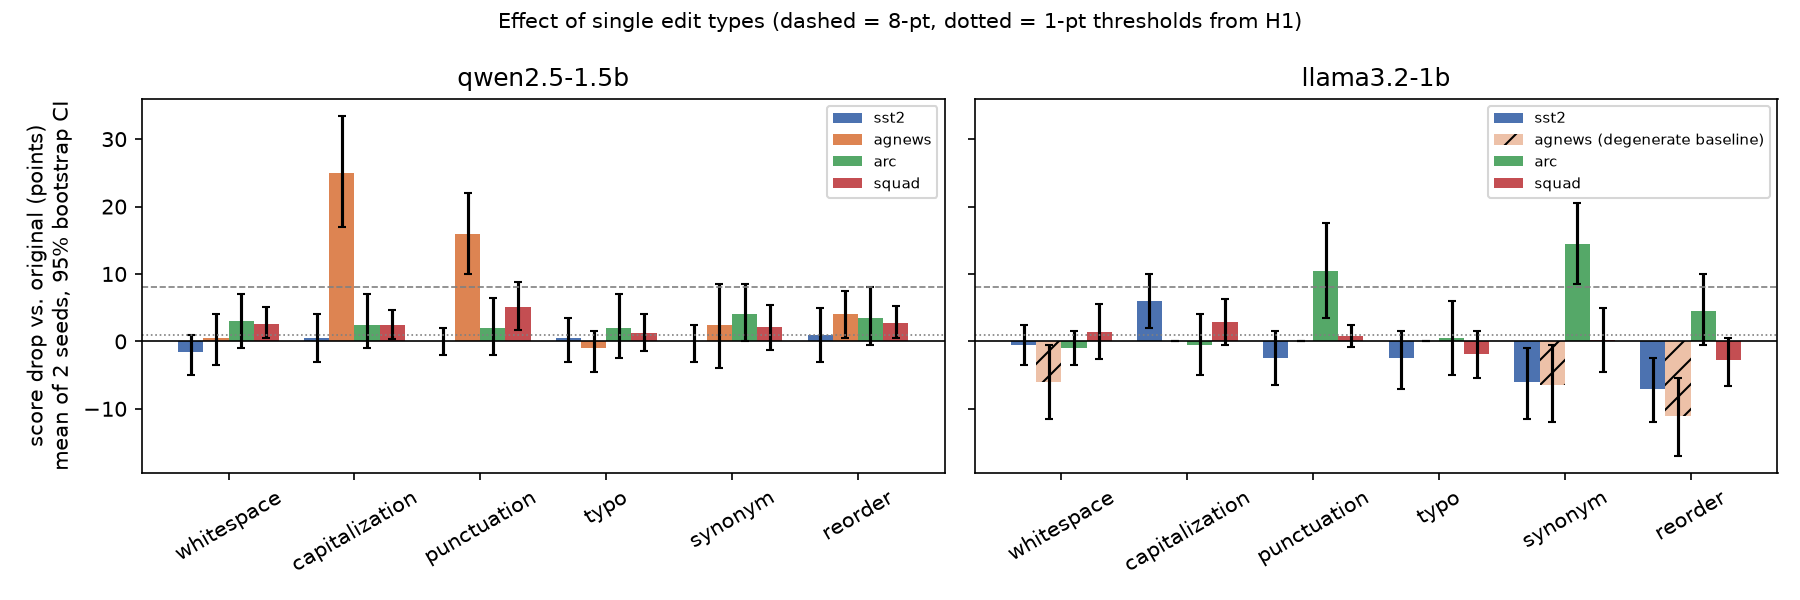
\includegraphics[width=0.95\linewidth]{figures/edit_type_by_model.png}
\caption{Score drop for each single edit type, by task, for \qwen \figleft and \llama \figright (mean of 2 seeds; error bars are 95\% bootstrap CIs). The dashed and dotted lines mark H1's 8-point and 1-point thresholds. Only three cells are significant drops above 8 points, and none of them belongs to \reord. Negative bars are edits that \emph{improve} the score.}
\label{fig:h1}
\end{figure}

\Tabref{tab:h1} and \figref{fig:h1} report the drop caused by each single edit type, and \tabref{tab:h1_pooled} pools these drops over tasks. H1 predicted that \reord and \syn would cost more than 8 points while \ws and \caps would cost less than 1 point. The data refute both halves.

{\bf Which edits hurt?} The largest drops come from edits that H1 called harmless. For \qwen on \agnews, \caps costs 25.0 points (CI [17.0, 33.5]) and \punct costs 16.0 points (CI [10.0, 22.0]). Both survive Holm correction. The same two edits cost \qwen at most 0.5 points on \sst. For \llama, the largest drops are \syn on \arc (14.5 points) and \punct on \arc (10.5 points, not significant after correction). \Secref{sec:mechanisms} shows that the first is mostly a format effect and the second a content effect.

{\bf Which edits are safe?} \reord never costs more than 4.5 points on any valid task. It significantly \emph{improves} \llama on \sst (by 7.0 points) and on \agnews (by 11.0 points). \syn never costs \qwen more than 4.0 points. \typo is the most benign edit overall (at most 2.0 points). \ws is the only edit type whose effect is small on every valid task ($|\Delta| \leq 3$ points), although its \squad CI for \qwen lies just above the 1-point threshold.

{\bf Net drops understate churn.} The flip rate of an edit type ranges from 2--8\% in robust cells to 32\% for \qwen \agnews under \caps and 25.5\% for \llama \arc under \punct. Flip rates are often several times larger than the net $|\Delta|$, because the same edit fixes some items while breaking others (\figref{fig:flip} in \appref{app:figures}).

\begin{table}[t]
\centering
\small
\begin{tabular}{@{}lccp{0.34\linewidth}@{}}
\toprule
\textbf{Edit} & \qwen & \llama\ {\scriptsize(excl.\ \agnews)} & \textbf{Verdict on H1} \\
\midrule
\ws    & 1.2 (3.0)  & 0.0 (1.5)  & \textit{roughly supported} (small everywhere) \\
\caps  & {\bf 7.6} (25.0) & 2.8 (6.0) & \textit{refuted} (not below 1 point) \\
\punct & 5.8 (16.0) & 2.9 (10.5) & not in H1; large on some tasks \\
\typo  & 0.7 (2.0)  & $-$1.3 (0.5) & not in H1; robust \\
\syn   & 2.1 (4.0)  & 2.9 (14.5) & \textit{refuted} for \qwen; above 8 only for \llama on \arc (a format effect) \\
\reord & 2.8 (4.0)  & $-$1.8 (4.5) & \textit{refuted} (never above 8 points) \\
\bottomrule
\end{tabular}
\caption{Mean drop (points) over valid tasks, with the largest single-task drop in parentheses. The largest mean drop is in \textbf{bold}.}
\label{tab:h1_pooled}
\end{table}

\subsection{H2: generation is not the most fragile task type}
\label{sec:h2}

\begin{table}[t]
\centering
\small
\begin{tabular}{@{}llcc@{}}
\toprule
\textbf{Task} & \textbf{Type} & \qwen & \llama \\
\midrule
\sst    & classification  & 0.001 \ci{$-$0.03}{0.03} & $-$0.028 \ci{$-$0.07}{0.02} \\
\agnews & classification  & {\bf 0.104} \ci{0.06}{0.15} & (degenerate) \\
\arc    & multiple choice & 0.039 \ci{$-$0.01}{0.09} & {\bf 0.097} \ci{0.02}{0.18} \\
\squad  & generation      & 0.031 \ci{0.01}{0.05} & 0.002 \ci{$-$0.04}{0.04} \\
\midrule
\multicolumn{2}{@{}l}{Classification mean (H2 predicted 0.05)} & 0.053 & $-$0.028 \\
\multicolumn{2}{@{}l}{Generation (H2 predicted 0.22)} & 0.031 & 0.002 \\
\bottomrule
\end{tabular}
\caption{Mean \pfi over the 12 single-edit conditions of each task, with item-bootstrap 95\% CIs. The most fragile task for each model is in \textbf{bold}. Generation is far below the predicted 0.22 for both models.}
\label{tab:h2}
\end{table}

\begin{figure}[t]
\centering
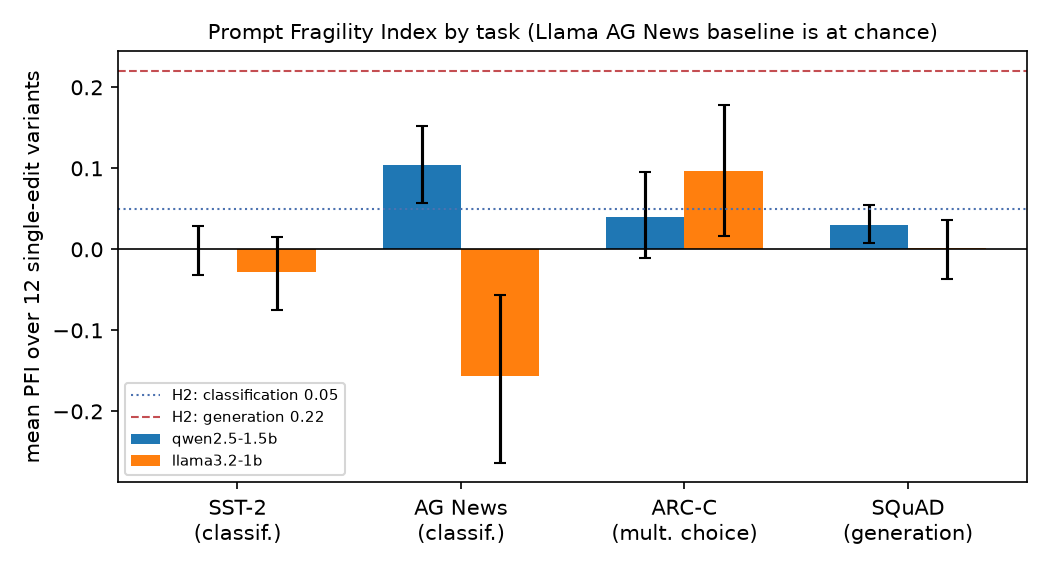
\includegraphics[width=0.62\linewidth]{figures/pfi_by_task_model.png}
\caption{Mean \pfi over the 12 single-edit conditions, by task and model, with 95\% bootstrap CIs. The dotted and dashed lines show the values H2 predicted for classification (0.05) and generation (0.22). The negative \llama \agnews bar comes from its chance-level baseline (edits break its first-label collapse) and is not a real robustness gain.}
\label{fig:h2}
\end{figure}

H2 predicted that classification would be the most robust task type (mean \pfi about 0.05) and generation the most fragile (about 0.22). \Tabref{tab:h2} and \figref{fig:h2} refute this. Generation has a mean single-edit \pfi of only 0.031 for \qwen and 0.002 for \llama. The most fragile task is \agnews for \qwen (0.104) and \arc for \llama (0.097). The classification mean for \qwen (0.053) matches the predicted 0.05 only as an average of a near-zero \sst (0.001) and a fragile \agnews. The two classification tasks lie at opposite ends of the range, which shows that task type is a poor predictor of fragility. Including the combined conditions raises \qwen's \squad \pfi to 0.081 [0.05, 0.11], because of the super-additive compounding we report next, but this is still below \agnews (0.190).

\subsection{H3: edits compound super-additively only for generation}
\label{sec:h3}

\begin{table}[t]
\centering
\resizebox{\textwidth}{!}{%
\begin{tabular}{@{}llcccccc@{}}
\toprule
\textbf{Task} & $k$ & $\Delta$ combined & Additive baseline & Ratio & Interaction vs.\ additive & Union baseline & Interaction vs.\ union \\
\midrule
\sst    & 3 & 0.8  & 0.7  & ---  & $+$0.2 \ci{$-$4.7}{5.7} & 4.0 & $-$3.2 \ci{$-$6.7}{$-$0.5} \\
\agnews & 3 & 21.0 & 26.2 & 0.80 & $-$5.2 \ci{$-$12.2}{1.7} & 27.7 & $-$6.7 \ci{$-$11.0}{$-$2.3} \\
\agnews & 6 & 36.0 & 47.0 & 0.77 & $-$11.0 \ci{$-$28.5}{6.5} & 43.0 & $-$7.0 \ci{$-$14.5}{0.5} \\
\arc    & 3 & 4.2  & 9.0  & 0.46 & $-$4.8 \ci{$-$13.2}{3.2} & 7.5 & $-$3.3 \ci{$-$6.8}{$-$0.2} \\
\arc    & 6 & 6.5  & 17.0 & 0.38 & $-$10.5 \ci{$-$30.0}{8.0} & 9.5 & $-$3.0 \ci{$-$8.0}{1.5} \\
\midrule
\squad  & 2 & 7.9  & 4.9  & {\bf 1.61} & $+$3.0 \ci{0.3}{5.9} & 5.5 & $+$2.4 \ci{$-$0.4}{5.1} \\
\squad  & 3 & 11.1 & 7.8  & {\bf 1.42} & $+$3.3 \ci{$-$2.2}{8.2} & 7.7 & $+$3.3 \ci{$-$0.6}{7.2} \\
\squad  & 6 & 20.9 & 16.2 & {\bf 1.29} & $+$4.7 \ci{$-$6.5}{15.0} & 10.7 & {\bf $+$10.2} \ci{4.3}{16.3} \\
\bottomrule
\end{tabular}%
}
\caption{Compounding for \qwen, pooled over all combinations with $k$ edit types and both seeds (points). Ratio is $\Delta$(combined) divided by the sum of single-edit drops (omitted for \sst, where both are near 0). Interaction CIs come from the item bootstrap. Super-additive results are in \textbf{bold}. Combined edits are super-additive only on \squad, and only \combo{all6} clearly exceeds the union baseline.}
\label{tab:h3}
\end{table}

\begin{figure}[t]
\centering
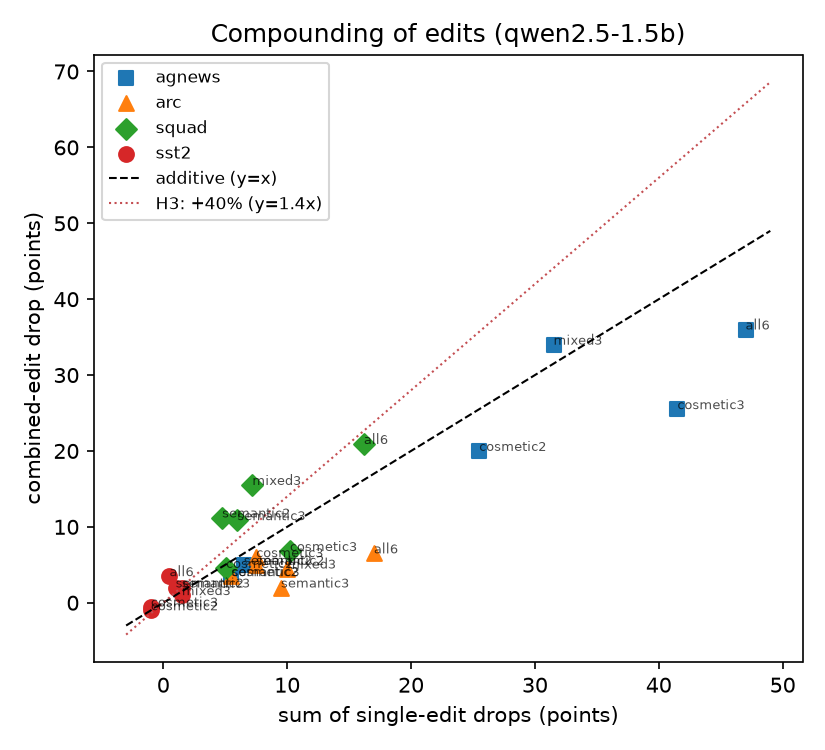
\includegraphics[width=0.5\linewidth]{figures/compounding_qwen2_5-1_5b.png}
\caption{Drop of each combined edit against the sum of the drops of its parts, for \qwen (each point is one combination at one seed). Points above the dashed line are super-additive; the dotted line is H3's $+$40\% prediction. Only \squad combinations (green) lie above the additive line. \agnews and \arc combinations lie below it, because items broken by one edit cannot break again.}
\label{fig:h3}
\end{figure}

H3 predicted that combining three or more edit types would exceed the sum of their individual effects by 30--50\%. \Tabref{tab:h3} and \figref{fig:h3} show the results for \qwen.

{\bf Generation compounds.} On \squad, combined edits exceed the additive baseline, with ratios of 1.61 for $k=2$, 1.42 for $k=3$ and 1.29 for $k=6$, close to the hypothesized range. The evidence is moderate, however. At $k=3$, the interaction CI includes 0 against both baselines. Only \combo{all6} clearly exceeds the union baseline ($+$10.2 points, CI [4.3, 16.3]).

{\bf Classification and multiple choice saturate.} On \agnews and \arc, combined edits are sub-additive, with ratios of 0.38--0.80. They break even fewer items than the union baseline predicts (for example $-$6.7 points, CI [$-$11.0, $-$2.3], for \agnews at $k=3$). The additive baseline overstates the no-interaction prediction because it counts an item broken by two edits twice. The negative union interaction means that a combination breaks fewer items than its parts do individually, which suggests that some edits partly cancel each other's damage.

{\bf \llama.} For \llama, the single-edit drops have mixed signs (for example, the sum of single drops on \sst is negative), so additive ratios are unstable. Against the union baseline, the interaction is negative in 5 of the 6 \sst and \squad cells, with all 5 CIs below 0. The exception is \sst \combo{all6} ($+$4.0, CI [$-$4.5, 12.5]). It is also negative in all three cells of the degenerate \agnews task. On \arc it is $-$3.8, $-$2.7 and $-$11.5 points for $k = 2$, 3 and 6. Individual \arc combinations can still be strongly super-additive: \combo{semantic3} at seed 0 loses 48 points against 33 for the sum of its parts, and \combo{mixed3} at seed 0 loses 40 against 26. \Secref{sec:format} traces these losses to output-format failures. Overall, H3 holds only for generation in one model.

\subsection{Larger edits cause more churn, not reliably more damage}
\label{sec:magnitude}


The character-level edit distance between the original and edited instruction correlates with the flip rate for both models (Spearman $\rho = 0.46$ for \qwen and $0.51$ for \llama, $p < 10^{-5}$, $n = 96$ conditions). It correlates with the net drop only for \qwen ($\rho = 0.44$; $\rho = 0.02$ for \llama). Larger edits change more individual answers, but whether they lower the net score depends on what they touch.

\section{Discussion}
\label{sec:discussion}

\subsection{Why do ``cosmetic'' edits break classification?}
\label{sec:mechanisms}

\begin{table}[t]
\centering
\small
\begin{tabular}{@{}lcccc@{}}
\toprule
\textbf{Condition} & Business & World & Sports & Sci/Tech \\
\midrule
original & 42 & 26 & 21 & 11 \\
\caps, seed 0 (all lowercase) & 29 & 12 & 12 & {\bf 46} \\
\caps, seed 1 (random case) & 42 & {\bf 4} & {\bf 42}$^\ast$ & 10 \\
\punct, seed 0 (commas removed) & 23 & {\bf 55} + 10$^\ddagger$ & 3 & 9 \\
\bottomrule
\end{tabular}
\caption{Predicted-label counts for \qwen on \agnews (out of 100 items). Edits to the casing or punctuation of the label list shift the model's label preferences, and removing the commas makes ``World Sports'' look like a single label. Large shifts from the original distribution are in \textbf{bold}. $^\ast$Includes re-cased outputs such as ``SPOrts''. $^\ddagger$Outputs of the merged label ``World Sports''.}
\label{tab:labels}
\end{table}

\Tabref{tab:labels} shows how \qwen's predictions on \agnews change under the two damaging edits. The edits do not change the task wording; they change the \emph{answer-space specification}. Removing the commas from ``World, Sports, Business, and Sci/Tech'' turns the list into ``World Sports Business and Sci/Tech:'', and the model then predicts ``World'' 55 times and ``World Sports'' 10 more times. Lowercasing the list moves predictions toward ``sci/tech'' (11 $\to$ 46). Random re-casing nearly removes ``World'' (26 $\to$ 4) while doubling ``Sports''. These are content errors, not format errors: accuracy among parsed outputs falls from 75\% to 50--60\%. The two-label \sst instruction (``positive or negative'') survives the same edits unharmed. Fragility therefore follows the size and delimitation of the label set more than the edit category. A taxonomy that labels capitalization and punctuation as cosmetic misses that these edits can rewrite the part of the prompt that defines the possible answers.

\subsection{Why is generation not the most fragile, yet the only one that compounds?}

The \squad instruction states its format constraint twice: the answer is ``a short span copied directly from the passage'', and the model should give ``only the answer span, without any explanation''. A single edit rarely removes both, so single-edit drops stay small (\pfi 0.03). Under the \combo{semantic2}, \combo{semantic3}, \combo{mixed3} and \combo{all6} combinations, \qwen's mean answer length grows from 3.0 to 4.8--7.3 words, and exact match falls from 0.77 to 0.40--0.61. The model starts answering in full sentences, for example ``John Myhill'' becomes ``John Myhill provided a definition of linear bounded automata in 1960.'' Each edit weakens the format constraint a little, and only together do they cross the point where the model abandons span-style answers. This is a plausible mechanism for the super-additivity we see only on generation. It also explains the contrast with classification: classification scores are bounded per item, so once an item is wrong it cannot get more wrong, and combined effects saturate.

\subsection{Format fragility versus content fragility}
\label{sec:format}

\begin{table}[t]
\centering
\small
\begin{subtable}[t]{0.47\linewidth}
\centering
\resizebox{\linewidth}{!}{%
\begin{tabular}{@{}lcc@{}}
\toprule
\textbf{Condition} & Parse failures & Acc.\ among parsed \\
\midrule
original    & 4\%  & 51\% \\
\syn        & {\bf 32\%} & 51\% \\
\punct      & 2\%  & {\bf 39\%} \\
\combo{semantic3} & {\bf 48\%} & 38\% \\
\combo{mixed3}    & {\bf 44\%} & 37\% \\
\bottomrule
\end{tabular}}
\caption{Strict scoring, 8-token budget (both seeds).}
\label{tab:format_a}
\end{subtable}
\hfill
\begin{subtable}[t]{0.5\linewidth}
\centering
\resizebox{\linewidth}{!}{%
\begin{tabular}{@{}lccc@{}}
\toprule
\textbf{Condition} & 8 tok., strict & 48 tok., lenient & Unparsed \\
\midrule
original          & 49 & 50 & 3\% \\
\syn, seed 0      & 21 & 44 & 18\% \\
\combo{semantic3}, seed 0 & 1 & 40 & 16\% \\
\combo{mixed3}, seed 0    & 9 & {\bf 52} & 6\% \\
\bottomrule
\end{tabular}}
\caption{Accuracy (\%) re-scored with a 48-token budget and a lenient parser.}
\label{tab:format_b}
\end{subtable}
\caption{Format versus content fragility for \llama on \arc. \captiona The \syn drop comes entirely from parse failures (accuracy among parsed outputs is unchanged at 51\%), while the \punct drop is a genuine content effect. \captionb With a generous budget and a lenient parser, most catastrophic drops disappear.}
\label{tab:format}
\end{table}

Not every drop means the model got the answer wrong. \Tabref{tab:format}a splits \llama's \arc results into parse failures and accuracy among parsed outputs. The \syn edit rewrites ``Choose the single best answer'' as ``Pick the single most suitable answer'', and the model echoes this phrase as a preamble, which the 8-token budget cuts off before the letter. When the persona sentence is also moved (\combo{semantic3}, \combo{mixed3}), the model often opens with ``As a science teacher, I'd\dots''. Parse failures rise from 4\% to 32\%, while accuracy among parsed outputs stays at 51\%. The \syn drop is therefore entirely a format effect. The \punct drop, by contrast, comes with almost no parse failures and a 12-point fall in accuracy among parsed outputs, so it is a content effect.

To measure how much of the format effect is truncation, we re-ran four \llama \arc conditions with a 48-token budget and a lenient extractor that also accepts patterns such as ``answer is X'' and ``option X'' (\tabref{tab:format}b). The original prompt barely changes (49 $\to$ 50). The catastrophic drops largely disappear: \combo{semantic3} recovers from 1\% to 40\% and \combo{mixed3} from 9\% to 52\%. A residual drop of 6--10 points remains for \syn and \combo{semantic3}, partly from answers that still have no letter within 48 tokens. Fragility is therefore partly a property of the \emph{evaluation protocol}. Strict, short-budget scoring matches what the prompt asks for (``only the letter''), but it inflates format-driven \pfi for weaker instruction followers. We encountered this issue ourselves. A pilot with a 3-token budget for \arc gave 14\% parse failures even for the \emph{original} prompt, because outputs such as ``The correct answer\dots'' were cut off. We discarded that run before any analysis and re-ran \arc with 8 tokens.

\subsection{Edits can help}
\label{sec:edits_help}

Several edits significantly \emph{improve} accuracy. For \llama, \reord adds 7.0 points and \syn adds 6.0 points on \sst. On \agnews, \reord adds 11.0 points from the degenerate baseline: moving the label sentence away from its original position weakens the model's collapse onto the first-listed label ``World'', a bias related to those described by \citet{zhao2021calibrate}. The original wording is not privileged; it is one sample from a distribution of equivalent prompts, as \citet{mizrahi2024state} argue. Signed averages of \pfi can hide such gains, which is why we also report $|\pfi|$ and flip rates.

\subsection{Limitations}
\label{sec:limitations}

\para{Small models only.} We could not evaluate hosted frontier models because no API key was available, and the host had no GPU. Both models have 1--1.5B parameters and run at Q8\_0 quantization, which is near-lossless but not identical to bf16. Fragility generally decreases with scale and better instruction tuning, so our magnitudes should be read as upper-range values and not extrapolated to frontier models.

\para{Statistical power.} With $n = 100$ items per task and 2 seeds per edit type, effects of 4--5 points often fall inside the CI. Only 5 of 48 edit $\times$ task cells survive Holm correction (4 excluding the degenerate \llama \agnews cell). More seeds would better separate the effect of an edit \emph{type} from that of a particular random edit.

\para{One template per task.} Several effects come from specific template features, such as the comma-delimited label list or the persona sentence. Other base prompts could rank the edit types differently. Our results suggest that the ranking depends more on prompt structure than on edit category, but testing this requires several templates per task.

\para{Task-type confound.} Each task type has only one or two tasks, so differences between types are confounded with dataset, label-set size, baseline accuracy and metric (\squad's F1 is continuous rather than binary).

\para{Scoring protocol and noise.} Strict short-budget scoring inflates format-driven fragility (\secref{sec:format}), and we quantified this only for \llama on \arc. llama.cpp batching changed about 5\% of identical requests (0--2\% correctness flips), so effects of 2 points or less are within noise. The exclusion of \llama \agnews was decided post hoc.

\para{Edit design.} The synonym lexicon and typo rates are our own choices. We checked meaning preservation by inspection rather than with human raters, and a few substitutions are slightly ungrammatical (\eg ``an specialist'').

\subsection{Broader implications}
Our results matter for anyone who reports benchmark numbers or maintains production prompts. Single-prompt evaluation can over- or under-state a model by 10--25 points for a small model, depending on details that look irrelevant. Edits to the parts of a prompt that define the answer space or the output format deserve the same regression testing as code changes. Conversely, our finding that some edits help suggests that reported scores reflect partly the prompt author's luck. We see no direct risk of misuse: the edits we study are benign by design and are much weaker than existing adversarial attacks.

\section{Conclusion}
\label{sec:conclusion}

We asked how much small, meaning-preserving edits to an instruction change LLM task performance. To answer it, we built a controlled protocol: six benign edit types, a seeded editor whose combined edits reuse the local edits of their parts, and a paired item-level analysis with flip rates and additive and union baselines. Across two small instruction-tuned models, four tasks and 20,800 scored generations, a single edit typically moves scores by 0--5 points, but specific edit--task pairs move them by 10--25 points. The damaging edit is not a fixed edit type. Edits that alter the answer-space specification, such as the punctuation and casing of a label list, break classification. Edits that weaken the output-format constraint break strict-format multiple choice and, when combined, generation. Generation was not the most fragile task type, and super-additive compounding appeared only there. Elsewhere, effects saturate because an item can break only once.

{\bf Key takeaway:} prompt fragility follows what an edit touches, not what kind of edit it is. Label lists and output-format instructions are load-bearing parts of a prompt. Sensitivity metrics should be reported together with the parser and token budget used, and with flip rates rather than only net changes.

\para{Future work.} The most important next step is to repeat the study with frontier models, which only requires pointing our code at a hosted endpoint. We also plan to use several base templates per task, to separate edit type from template structure, and to run more seeds per edit type. Adding a lenient or LLM-judge scorer to every condition would separate format and content fragility throughout. Longer-form generation, such as summarization and chain-of-thought math, would test whether compounding grows with output length. Finally, a targeted experiment that edits only the label list or only the task description would directly test the answer-space mechanism.


\bibliography{references}

\appendix
\section{Instruction templates}
\label{app:prompts}

\Tabref{tab:prompts} lists the four original instructions. Each prompt is the instruction, a blank line and the task input, prefixed with \texttt{Review:}, \texttt{Article:}, \texttt{Question:} (followed by lettered options) or \texttt{Passage:} \dots\ \texttt{Question:}. Words in the protected column are never changed by \syn or \typo edits.

\begin{table}[h]
\centering
\small
\renewcommand{\arraystretch}{1.2}
\begin{tabular}{@{}p{0.11\linewidth}p{0.63\linewidth}p{0.2\linewidth}@{}}
\toprule
\textbf{Task} & \textbf{Instruction (four sentences)} & \textbf{Protected words} \\
\midrule
\sst & You are an expert sentiment analysis assistant. Read the movie review provided below carefully. Determine whether the overall sentiment expressed in the review is positive or negative. Answer with exactly one word: positive or negative. & positive, negative \\
\agnews & You are an expert news topic classifier. Read the news article provided below carefully. Decide which topic the article belongs to; the possible topics are World, Sports, Business, and Sci/Tech. Respond with only the topic name and nothing else. & World, Sports, Business, Sci/Tech \\
\arc & You are a knowledgeable science tutor. Read the multiple-choice question provided below carefully. Choose the single best answer from the options. Respond with only the letter of the correct option (A, B, C, or D). & A, B, C, D \\
\squad & You are a precise reading comprehension assistant. Read the passage provided below carefully and then answer the question about it. The answer is a short span copied directly from the passage. Respond with only the answer span, without any explanation. & (none) \\
\bottomrule
\end{tabular}
\caption{Original instructions. Each has a persona sentence, a reading directive, a task definition and an output-format constraint.}
\label{tab:prompts}
\end{table}

\section{Implementation and reproducibility}
\label{app:impl}

We used llama.cpp \texttt{llama-server} (build b11624) on CPU with the Q8\_0 GGUF files \texttt{bartowski/Qwen2.5-1.5B-Instruct-GGUF} and \texttt{bartowski/Llama-3.2-1B-Instruct-GGUF}. Items were sampled with a fixed seed (42). The full run took about 2.3 hours of wall-clock time on up to four concurrent servers (6--8 threads each) on a shared 32-core host, with no API cost. In total we scored 2 models $\times$ 4 tasks $\times$ 26 conditions $\times$ 100 items $=$ 20,800 generations. We logged every prompt and response. Among 212 accidentally duplicated \squad requests for \llama, 95\% produced byte-identical outputs, which matches the noise floor in \tabref{tab:baselines}.

\section{Additional figures}
\label{app:figures}

\begin{figure}[h]
\centering
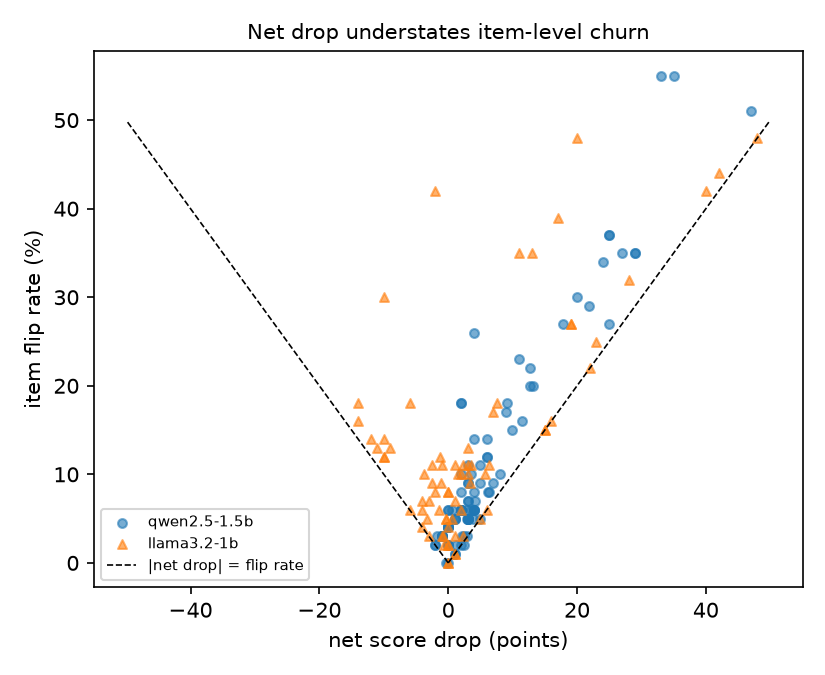
\includegraphics[width=0.55\linewidth]{figures/flip_vs_delta.png}
\caption{Item flip rate against net score drop for all 96 perturbed condition--task pairs of each model. Points on the dashed V have no churn beyond the net change. Most points lie well above it: edits fix some items while breaking others, so a small net change can hide a flip rate above 40\%.}
\label{fig:flip}
\end{figure}


\begin{figure}[h]
\centering
\begin{subfigure}[b]{0.49\textwidth}
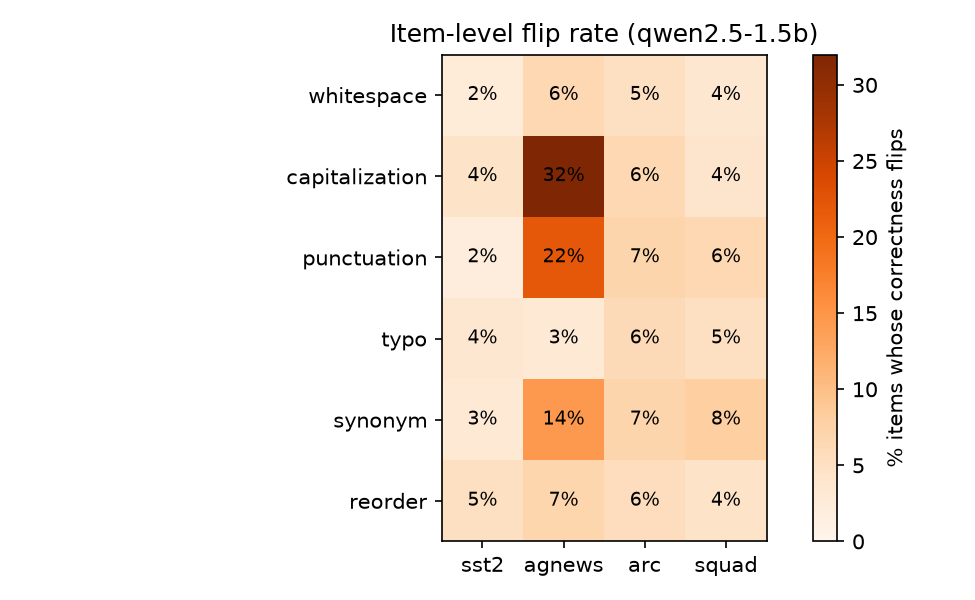
\includegraphics[width=\textwidth]{figures/heatmap_flip_qwen2_5-1_5b.png}
\caption{\qwen}
\end{subfigure}
\hfill
\begin{subfigure}[b]{0.49\textwidth}
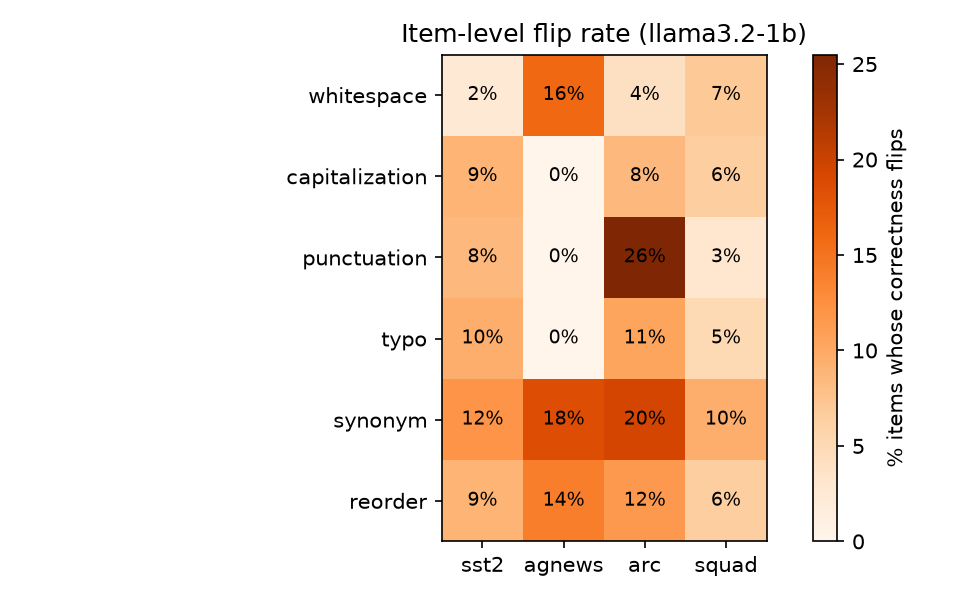
\includegraphics[width=\textwidth]{figures/heatmap_flip_llama3_2-1b.png}
\caption{\llama}
\end{subfigure}
\caption{Item flip rate for every condition and task. Flip rates are often several times larger than the net score change in \tabref{tab:h1}.}
\label{fig:heat_flip}
\end{figure}

\begin{figure}[h]
\centering
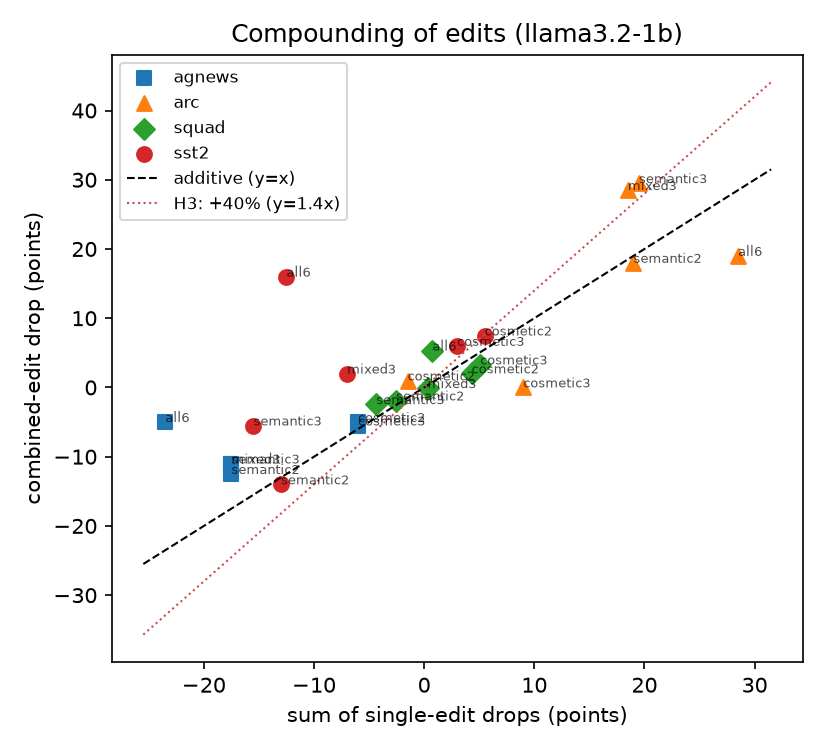
\includegraphics[width=0.6\linewidth]{figures/compounding_llama3_2-1b.png}
\caption{Drop of each combined edit against the sum of its parts for \llama. Because single-edit drops have mixed signs, the additive ratio is unstable for this model; \secref{sec:h3} reports the union-baseline analysis.}
\label{fig:h3_llama}
\end{figure}


\end{document}
